\documentclass[print]{uit-thesis}

\usepackage[backend=bibtex,style=numeric,sorting=none]{biblatex}
\usepackage{gensymb}
\usepackage{pgfplots}
\usepackage{pgfplotstable}
\usepackage{tikz}
\usepackage[toc,page]{appendix}
\usepackage{adjustbox}
\usepackage{tabularx}
\bibliography{main}
\usepackage[utf8]{inputenc}

\graphicspath{{images/}}

% Define colours
\definecolor{bblue}{HTML}{72A9DA}
\definecolor{rred}{HTML}{CA422D}
\definecolor{ggreen}{HTML}{95C380}

\begin{document}

%:-------------------------- Frontpage ------------------------

\title{GeneNet VR: Large Biological Networks in Virtual Reality Using Inexpensive Hardware}
\subtitle{}% Note: this is optional, and may be commented out
\author{\'Alvaro Mart\'inez Fern\'andez}
\thesisfaculty{Faculty of Science and Technology \\ Department of Computer Science}
\thesisprogramme{INF-3990 Master's thesis in Computer Science - November 2020}

\pgfplotsset{width=\textwidth}

\maketitle

%:-------------------------- Frontmatter -----------------------
\frontmatter

%: Commented out
% \iffalse
% \begin{dedication}
% To...
%
% Thanks for...
% \end{dedication}

\begin{epigraph}
\epigraphitem{Anything created by human beings is already in the great book of nature.}{Antoni Gaudi}
\epigraphitem{There are decades of innovations ahead. We’re at the very beginning, where it’s just at the stage where we can bring in consumers [but] there’s so much further to go from there.}{Brendan Iribe}
\end{epigraph}

\begin{abstract}
Biological data is often visualized using networks. However, these networks face problems such as information overload, high interconnectivity, and high dimensionality. Existing approaches try to solve these problems by reducing the interactivity in favor of presenting more information or by using expensive hardware. This thesis aims to solve them using Virtual Reality (VR) and the Oculus Quest, an affordable VR headset, by taking advantage of the rich interactivity that VR offers.

In order to test our hypothesis that Virtual Reality can be advantageous in the visualization of large biological networks, we built GeneNet VR, an open-source prototype of a VR application for the Oculus Quest for the interactive visualization of large biological networks. As a case study, we used two gene networks from MIxT, a real application that uses a 2-dimensional network visualization. We evaluated the performance and scalability of GeneNet VR and we conducted in-depth semi-structured interviews with several research scientists to evaluate the usability of our approach.

Our result shows that the performance of the interactions for network visualization on a machine, reaches the 72 FPS required by the Oculus' performance guidelines and that GeneNet VR scales for our largest network with 2693 nodes. We also evaluated the performance of GeneNet VR on the Oculus Quest hardware, which also achieved 72 FPS. The Oculus Quest is therefore an affordable option for the visualization of large datasets. From the interviews, we learned that GeneNet VR is an innovative and interesting visualization tool for large biological networks and that is easy to use even for novice VR users. Thus, VR hardware like the Oculus Quest should be considered a competitive solution for visualization tools, as described in this thesis.

GeneNet VR is open-source and can be accessed with the following link: \url{https://github.com/kolibrid/GeneNet-VR}. We created also a video to show the different interactions that we can do with GeneNet VR to explore large biological networks: \url{https://www.youtube.com/watch?v=\_Iqa3yizYZ4}.

\end{abstract}

\begin{acknowledgement}

I would first like to thank my advisor, Associate Professor Edvard Pedersen, for his guidance through this thesis, his constant encouragement, and for the interesting discussions about Virtual Reality and Computer Science. I would also like to thank my co-advisor, Lars Ailo Bongo, for his great knowledge in Bioinformatics, his good criticism, and for all the great insights about scientific writing. Thank you also Vanessa Dumeaux, for introducing me to MIxT and for your great contributions to Biology.

I would also like to thank the collaboration of the several research scientists that participated in the evaluation of my project and that contributed to their knowledge in Biology and Computer Science.

To my close friends Juncal García García, Mireia Nager and Reidar Staupe-Delgado for all the great experiences in Tromsø and for teaching me the value of science.

To Ramsalt Lab, for making it possible for me to study and expand my knowledge in Computer Science.

I would like to thank also my family, for their support and encouragement even from the distance.

Finally, thank you Dominic Ochotorena for your love, for always supporting me, and for being there.

\end{acknowledgement}
% \fi
%: End comments

\tableofcontents

%:-------------------------- Mainmatter -----------------------
\mainmatter

\chapter{Introduction}
It is very cheap nowadays to produce data and many people are doing it due to technological advancement. Just as an example, in the field of genomics, the sequencing of the first human genome (2002) took around 13 years and cost over \$3 million to complete. Now we can sequence hundreds of genomes in a few days\cite{big_biological_impacts_bd}. This leads to the accumulation of vast quantities of genomic data, which can be used for new scientific discoveries, diagnose of rare diseases, etc. However we still need a human expert to visually inspect the data to find new signals and discover interesting patterns or to set a diagnosis. No matter how much resources we use into extracting the data if we don't get anything interesting out of it\cite{zhang_paciorkowski_craig_cui_2019}. Therefore there is a great need for new and better tools to support this task.

Some of the main problems that researchers face when analysing genomic data are information overload, data interconnectivity and high dimensionality. One way to deal with all this data is to invent novel analysis. However we still need visual inspection of the data, so the information overload still remains as an important challenge and this is what we attempt to solve. For this reason it is very important to implement efficient visualization technologies that can lead to find new patterns and the extraction of good conclusions of the data. In the field of system biology there are usually network representations where the nodes or bioentities are connected to each other, where these edges represent associations. Networks can increase dramatically in size and complexity and this is due to computational power to create very large networks, scientific knowledge about large networks and the big amounts of data that we have to analyze. We need therefore better visualization systems for the analysis and inspection of these networks.

In Figure \ref{fig:network_biology_evolution} we can see a representation of the evolution for visualization of networks in system biology. Before the computers, networks were represented in 2 dimensions and they were static representations that lacked interactivity, see Figure \ref{fig:network_biology_evolution} A. With the computer era and the advancement in computer graphics, 3D representations were possible, with the addition of interactivity with the network (See Figure  \ref{fig:network_biology_evolution} C). As computer science progressed, there was a big improvement in visualization and also new technologies emerged like virtual reality, which has a huge potential with regards to the interactivity (Figure \ref{fig:network_biology_evolution} I).

\begin{figure}[h!]
    \newlength{\tempheight}
    \setlength{\tempheight}{15ex}
    \centering%
    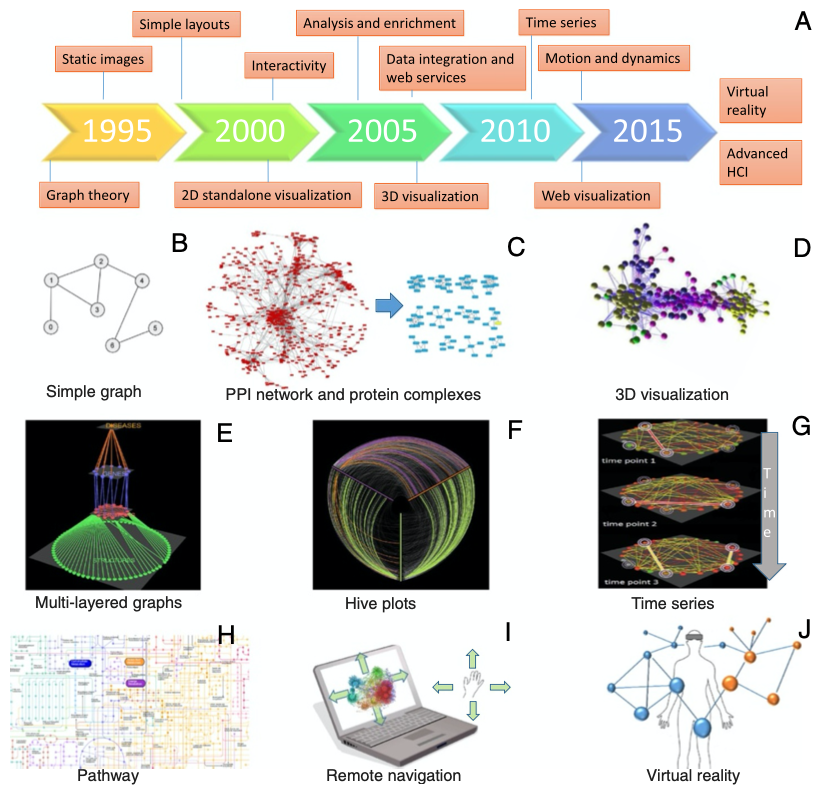
\includegraphics[width=\textwidth]{evolution_visualization}
    \caption{Visualization for network biology. a Undirected unweighted graph showing co-expression relationship between genes. b A 2D representation of a yeast protein-protein interaction network visualized in Cytoscape (left) and potential protein complexes 3D identified by the MCL algorithm from that network (right). c A 3D network of genes showing co-expression relationships. d A multilayered network integrating different types of data visualized by Arena3D. e A hive plot view of a network where nodes are mapped to and positioned on radially distributed linear axes. f Visualization of network changes over time. g Static picture showing part of lung cancer pathway. h Navigation of networks using hand gestures. i Integration and control of 3D networks using VR devices. Figure adapted\cite{pavlopoulos_malliarakis_papanikolaou_theodosiou_enright_iliopoulos_2015}.}
    \label{fig:network_biology_evolution}
\end{figure}%

We believe that virtual reality (VR) can offer new possibilities for visual inspection in large networks. Even though VR is still a field under exploration, it has been demonstrated that it help scientists work more effectively in fields like medicine \cite{Laver11}\cite{xia_ip_samman_wong_gateno_wang_yeung_kot_tideman_2001}\cite{brain_damage_rehab}, biology\cite{10.1093/bioinformatics/bti581}\cite{thorley_lawson_duca_shapiro_2008} and neuroscience\cite{bohil_alicea_biocca_2011}\cite{minderer_harvey_donato_moser_2016}, to  cite some examples. VR can be very powerful because it takes advantage of the way the human being perceives and analysis things. We have a great ability to discover patterns, however we are biologically optimized to see the world and the patterns in 3 dimensions. Some of the advantages that VR has over non-VR approaches are the following:

\begin{enumerate}
  \item Visualization of the network in a 3D space.
  \item Possibility to move around the virtual environment and visualize the network from different perspectives as in real life.
  \item Interaction with the the environment by using controllers and our virtual hands in the virtual world.
\end{enumerate}

We have implemented a virtual reality application for the visualization of 3-dimensional networks of data. We have used  up-to-date virtual reality techniques that we think it improves the visualization of this type of data structures. The techniques that we have used consist in: the exploration of the network by moving around the virtual space, making it easier for the user to see the network from different angles; interaction with the network and nodes to comprehend better the data that is being visualized; and the use of 2-dimensional user interfaces to filter and have more control of the data.

What did we learn... [Write when the evaluation is finished].

\textbf{Thesis statment: } \emph{Virtual reality techniques can improve the visualization and interactivity of data networks.}

\section{Challenges and research problem}
This project focus mainly on solving the problem of visualization of high dimenasional data from the MIxT project by using virtual reality. Furthermore the application allows the user to interact with the network created from the data in the virtual environment. It also allows the user compare the blood and biopsy networks at the same time in order to finde relationship, which wasn't possible in the MIxT web application as this only allows the user to visualize one network at a time.

MIxT\cite{fjukstad_dumeaux_olsen_lund_hallett_bongo_2017} is a web application for bioinformaticians. Among other tools, it offers a network visualization of genes which are represented as nodes in the network and where the edges represent statistically significant correlation in expression between two nodes. This tool was used in a study\cite{dumeaux_fjukstad_interactions_tumor_blood} that identifies genes and pathways in the primary tumor that are tightly linked to genes and pathways in the systemic response of a patient with breast cancer.
When exploring a network in MIxT, it can be hard to understand the data and its relationships because there is too much data. This problem is easy to occur when there are too many node and edges. In figure \ref{fig:mixt_network} we can see an example of the network visualization from MIxT. As we can see in Figure \ref{fig:mixt_network1}, there are many nodes and relationships among them and when we zoom in in the network, it becomes very difficult to understand the data and the relationships as shown in in Figure \ref{fig:mixt_network_zoom}.

 The network is also in 2-dimensions and what we propose in this project is to use a virtual reality 3d visualization in order to cope better with this problem.

\begin{figure}[h!]
    \centering%
    \begin{subfigure}[t]{0.5\textwidth}
        \centering%
        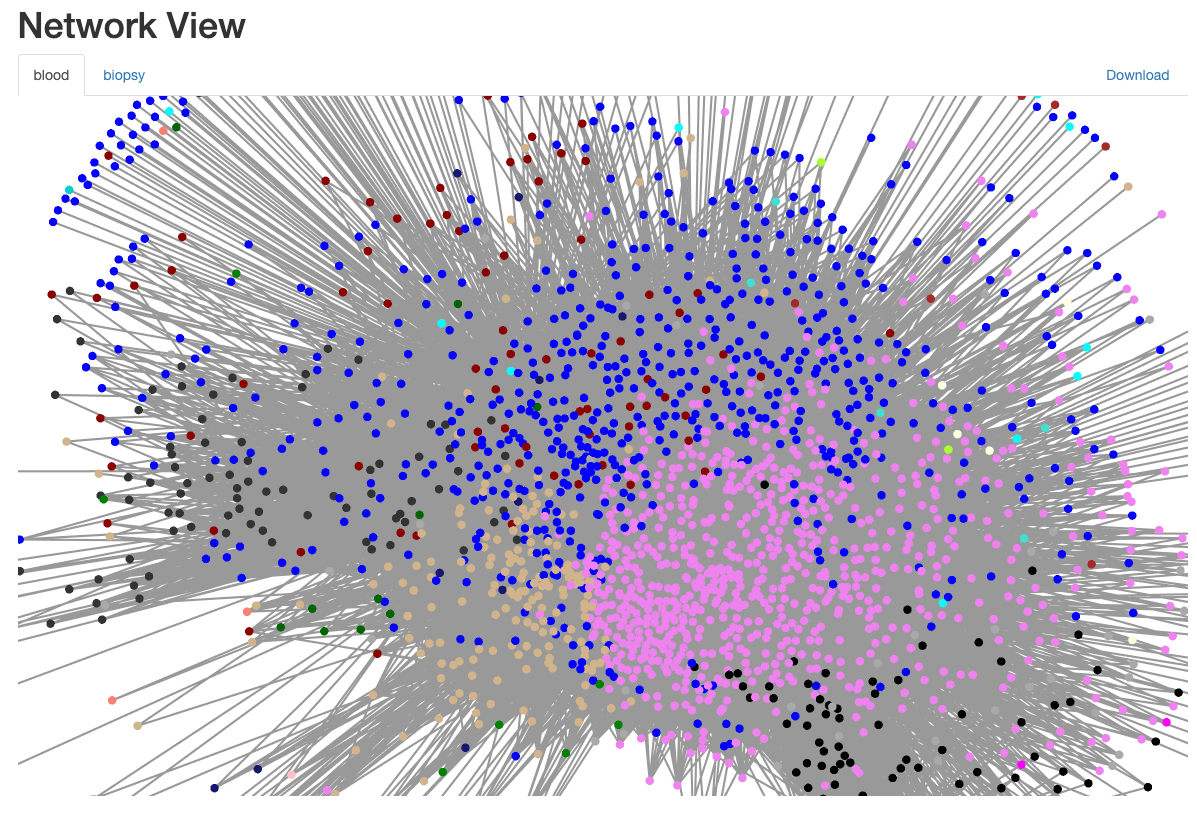
\includegraphics[width=\linewidth]{mixt_network1}
        \caption{Network with several modules.}
        \label{fig:mixt_network1}
    \end{subfigure}%
    \begin{subfigure}[t]{0.5\textwidth}
        \centering%
        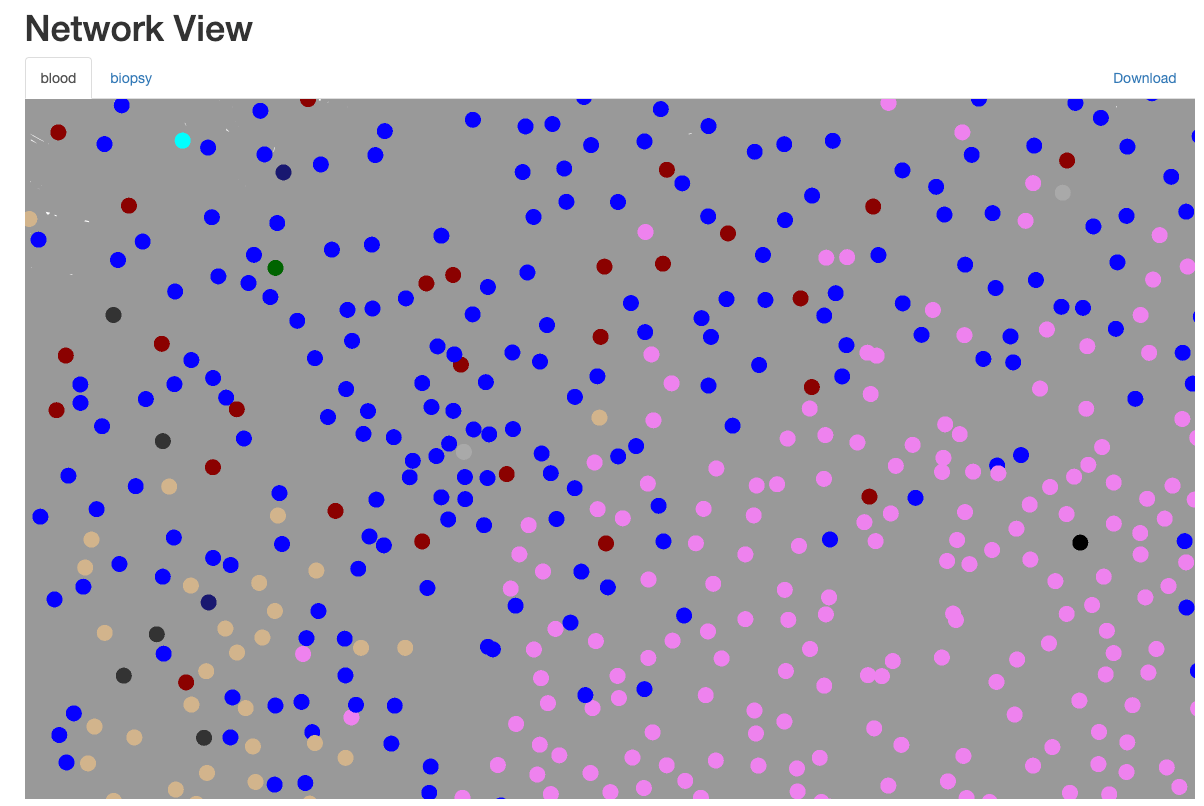
\includegraphics[width=\linewidth]{mixt_network2}
        \caption{Zoom in the network.}
        \label{fig:mixt_network_zoom}
    \end{subfigure}

    \caption{Network view of the MIxT application where nodes repsent genes and the modules are repsented by colors. Relationships are represented by grey lines that connect a gene with another one.}
    \label{fig:mixt_network}
\end{figure}

\section{Proposed solution}

\section{Significance and contribution}
This project contributes in the exploration of the possibilities that Virtual Reality offers for visualization of big data in bioinformatics.

\section{Outline}


\chapter{GeneNet VR}
%
% The points that I want to cover are the following:
%
% \begin{itemize}
%   \item Building the network from the bioinformatics data and clustering.
%   \item Manipulation of the network: translation and scaling.
%   \item Locomotion and ergonomics used in the VR environment.
%   \item Changing from the blood network to the biopsy network and viceversa.
%   \item Filtering genes in the network using gene sets that represent signatures of cellular pathways which are often dis-regulated in cancer.
% \end{itemize}

%In order to explore the network, several features have been implemented with the purpose of enhance the experience of the visualization process. For example the user has the possibility to move around the network by teleporting to a different place. It is also possible to translate the network and scale it, allowing the user have a better view of the data. The user can also point at a node using the controller to show the name corresponding to that gene or node. Another feature is about entering into a menu where the user can filter the network according to gene sets that represent signatures of cellular pathways which are often dis-regulated in cancer. And finally it is possible also to switch the network from a blood dataset to a biopsy dataset and viceversa.

%The genes nodes in the network and are represented as squared dots and the relationships are represented with lines between them. In Figure \ref{fig:bignet_vr} we can see an example of the application running.

GeneNet VR is a virtual reality application for the interactive visualization of gene networks in a 3D space. The network is represented by nodes for genes and edges for correlations between genes. In order to explore and visualize the data in GeneNet VR, the user can walk around the 3D environment, zoom in the network, translate (move from one place to another) the network, filter the nodes using a user interface, morph transition from one network to another and finally, also obtain detailed information about the nodes.

GeneNet VR loads the data from files resulting from bioinformatics analyses with the information about the nodes and relationships. Then the network is built using the data and clustered using an algorithm. Finally, the user can explore it and interact with it using the VR headset and controllers.

We implemented GeneNet VR in Unity, a cross-platform game engine. This software is used for a wide range of applications, eespecially for the development of videogames in 3D and 2D, VR applications, and engineering solutions. We used C\# as the main programming language to develop the application in Unity. We also used VRTK, a VR toolkit to build VR solutions in Unity. As for the VR hardware, we used an Oculus Quest headset. This type of headset is an all-in-one HMD, which means that it doesn't need to be connected to a PC to run an application, it has its own hardware to run the applications although this can be more limited than the hardware from a PC. Also, GeneNet VR is implemented on a platform where it is also possible to run it on a PC that has more computing power than the standalone headset.

We have used visualizations from MIxT as a case study. MIxT is a web application that is used for exploring and comparing bioinformatic data  \cite{fjukstad_dumeaux_olsen_lund_hallett_bongo_2017}  \cite{dumeaux_fjukstad_interactions_tumor_blood}. The datasets used here contain genetic information about a woman with breast cancer. There are in total 2 tissues; the first one is from a blood sample and the second one is from tumor tissue. The MIxT application has a visualization tool that has some issues, such as information overload and cumbersome interactions. In Figure \ref{fig:bignet_vr} we can see an example of GeneNet VR running using the blood dataset from MIxT. We will now detail how we implemented GeneNet VR.

\begin{figure}[h!]
    \setlength{\tempheight}{15ex}
    \centering
    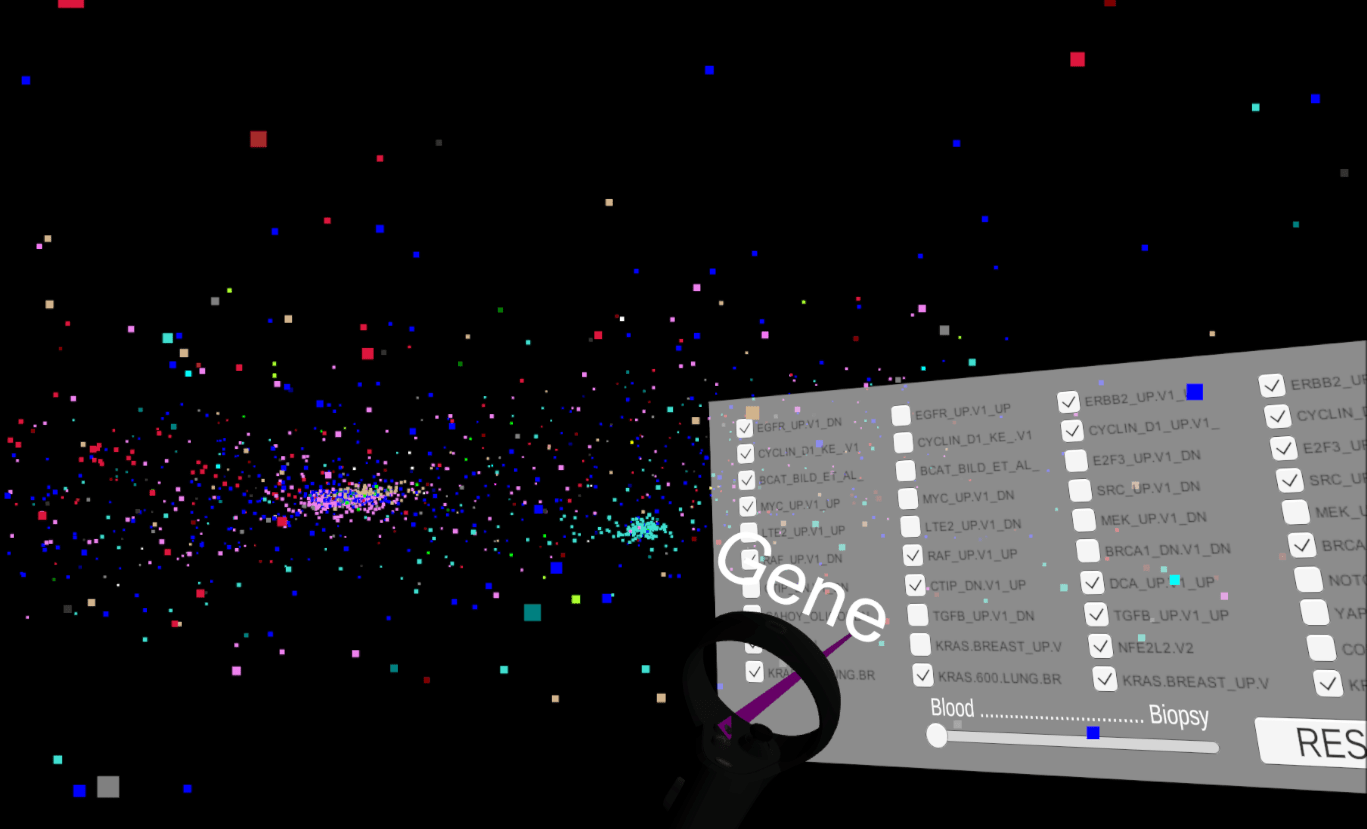
\includegraphics[width=\textwidth]{bignet_vr}
    \caption{Screenshot from GeneNet VR where a user explores a network.}
    \label{fig:bignet_vr}
\end{figure}

\section{Interaction with the network}
Virtual reality headsets offer a richly interactive and immersive experience. Some examples of what it is possible to do in virtual reality are for example moving around, grabbing objects, interact with the environment using your hands, controllers, or virtual tools, like pushing a button, 2D interfaces, and menus, etc. In this section, we will explain the techniques that we have implemented to visualize and interact with the network and make the most of VR.

The interaction and visualization depend on the VR technology used. We use Oculus Quest in this project, an all-in-one VR headset that doesn't need a PC nor wires to run the applications. Apart from the headset, it comes with 2 controllers; one for each hand. These controllers have inputs as buttons, thumbsticks, and triggers that can be used to activate actions in the VR application. We have used some of these inputs available in the controllers in GeneNet VR and mapped them to different actions that allow the user to interact with the network and the environment.

In Figure \ref{fig:oculus_quest_inputs} we can see which actions correspond to each input from the controllers. We will briefly explain now what these actions consist of 1. Snap rotation: It allows the user to instantly rotate to the right or to the left 45$^{\circ}$; 2. Filter and morph menu: The user can filter the nodes of the network according to a filtering algorithm used in GeneNet VR and also morph two networks; 3. Translate network: The network can be translated or moved to other positions in the scene; 4. Scale network: The network can be scaled or “zoomed”; 5. Select node: The user can select a node in order to get more information about it; 6. Select item in the menu: It allows the user to interact with the menu, for instance, to filter the nodes by enabling or disabling the checkboxes from the filtering menu; 7. Oculus menu: It opens the menu from oculus and pauses GeneNet VR; 8. Teleport: It teleports the user to another position on the floor of the VR scene.

As for the use of the Oculus Quest HMD (Head Mounted Display), this is placed in the head and it has a strap that is used to adjust the headset to the head. This will help the user feel more comfortable while wearing the HMD. Another important aspect that we have taken into account in GeneNet VR is that the user can use the application and explore the network by sitting on a chair. This is possible thanks to the locomotion techniques implemented that allows the user to move around with the controllers. We will go into more detail later in this chapter about this.

We will explain in the following subsections the different interaction techniques that we have used and also what benefits they bring for the visualization and interaction of the network.

\begin{figure}[h!]
    \centering%
    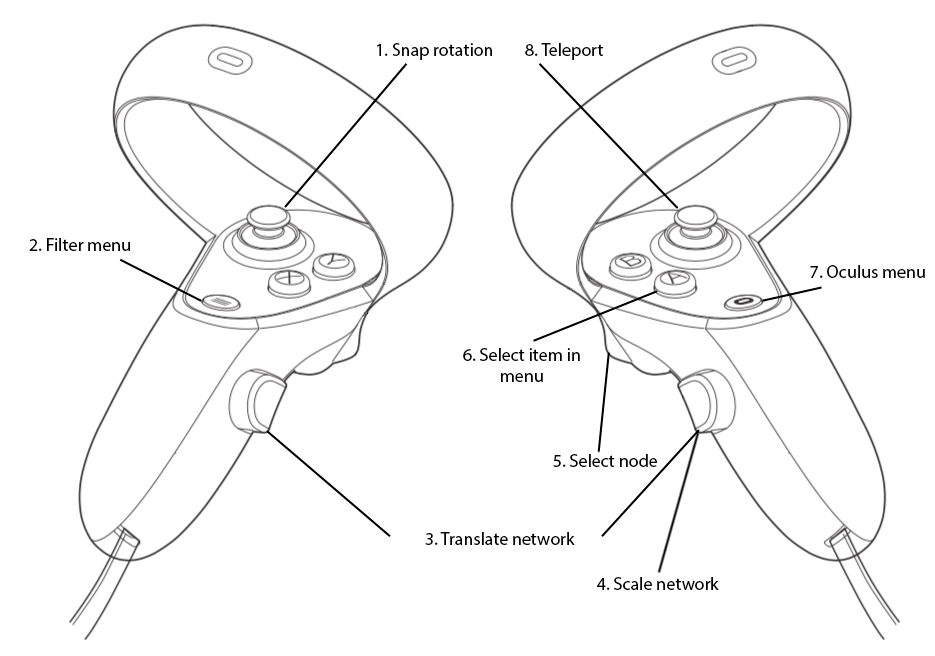
\includegraphics[width=\textwidth]{oculus_quest_inputs}
    \caption{Mapping of the Oculus Quest controllers for the different actions implemented in GeneNet VR: 1. Snap rotation. 2. Filter menu. 3. Scale environment. 4. Translate environment. 5. Pointer. 6. Select item in menu. 7. Oculus menu. 8. Teleport. Adapted figure from Oculus developer's page \cite{oculus_inputs}.}
    \label{fig:oculus_quest_inputs}
\end{figure}%

\subsection{Locomotion}
Locomotion is one of the most important ways of interaction in virtual reality experiences. It can be defined as a self-propelled movement in the virtual world. Even though moving around is not the main goal in most VR applications, it is an important aspect for the user's perspective in order to move the user's viewpoint in the virtual world and navigate around it.

Locomotion can have a strong influence on the user's experience. A poorly designed locomotion technique can reduce the user's immersion and even introduce motion sickness, which is related to the movement that the technique produces. HMDs like Oculus Quest allow the users to control the position and the orientation of the viewpoint by moving their heads and walking; however, large virtual environments such as GeneNet VR need a big physical tracked area, which cannot be covered by just walking around. It is for this reason that we need to use a locomotion technique that makes it possible to move around without having to walk around in the physical world \cite{locomotion_technique}. In addition, when the user is stationary both in the virtual and real world, the motion sickness produced by VR is less likely \cite{effect_vr_sickness}.

The locomotion technique that we use in GeneNet VR is called teleportation. It consists of choosing a spot on the floor where we want to teleport to. To do this the user has to move forward the thumbstick from the right controller (see “8. Teleport” from Figure \ref{fig:oculus_quest_inputs}). Furthermore, it is possible to choose which direction the user will face once the teleportation is completed. To do this we just need to rotate the same thumbstick to the desired direction. Once the user releases the thumbstick, a black flash will be followed by the new position in the space. This black flash is very important when implementing some of the locomotion techniques because it prevents producing motion sickness and disorientation. Without the black flash, the transition to the new position would be too abrupt and it may disorient the user.

\begin{figure}[h!]
    \centering%
    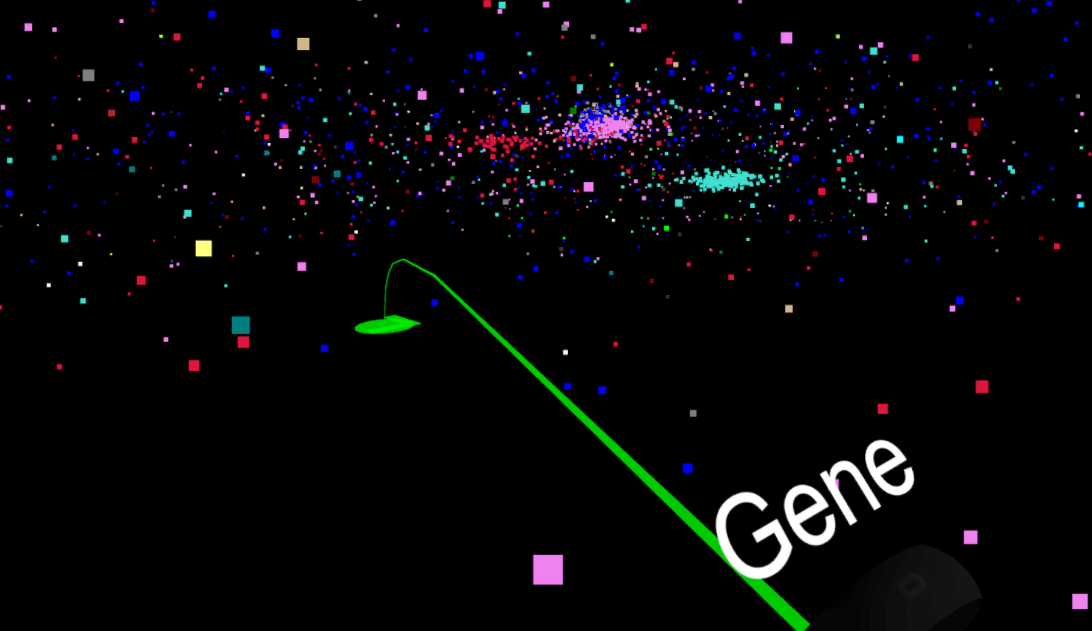
\includegraphics[width=\textwidth]{teleportation2}
    \caption{Teleportation technique. The user can use the jystick from the right controller to teleport to a different spot. To choose the spot a parabolic arc will appear.}
    \label{fig:teleportation}
\end{figure}%

In Figure \ref{fig:teleportation} we can see an example of how the teleportation technique is used in GeneNet VR. A  parabolic arc is created in the 3D space with a circle representing the spot where we are goin to teleport to. It can be seen as if we are throwing an object to the spot where we want to teleport to. The green circle includes also an arrow, indicating the direction that we will face once we are teleported.

In addition to the teleportation, it is also possible to rotate to the left or to the right with the Oculus controllers so that the user doesn't have to rotate the head to look around in the scene. This action is triggered using the thumbstick on the left hand (See 1. Snap rotation in Figure \ref{fig:oculus_quest_inputs}). By moving the thumbstick to the left side, the camera will rotate 45$^{\circ}$ to the left side, and 45$^{\circ}$ to the right side if the user moves it to the right side. A black transition is also used in this case before the rotation happens to avoid motion sickness, for the same reason as in the teleportation technique.

\subsection{Translation of the network}
By teleporting to different places in the environment, we allow the user visualize the network from different perspectives; however, it is also interesting to be able to move the network and especially move it in a precise way, so that the user has more control over what it is being visualized. The user might for instance be able to see the network or a specific node or cluster from above or also from below. To do this we have implemented functionality to translate the network in the 3D space.

\begin{figure}[h!]
    \centering%
    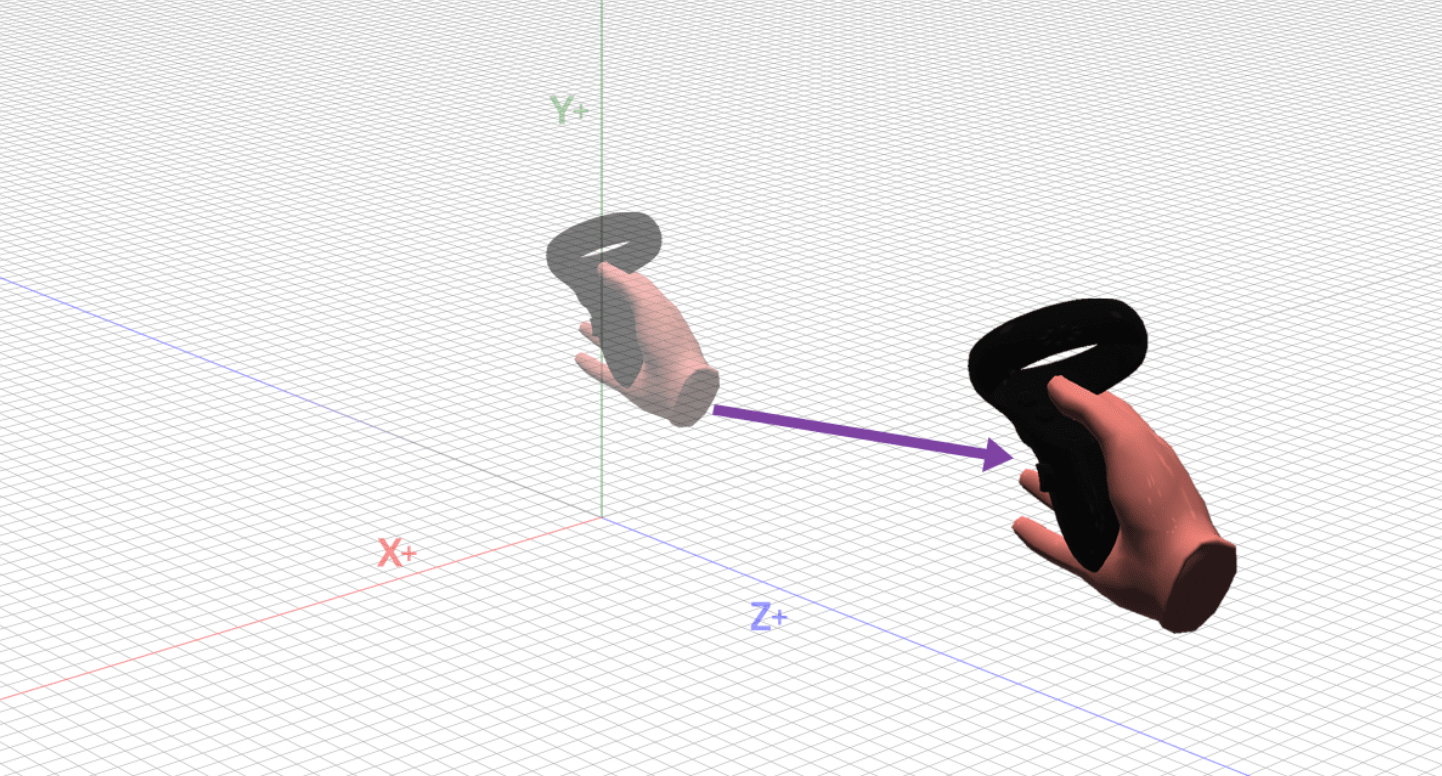
\includegraphics[width=\textwidth]{translation}
    \caption{Translation of the network functionality. The user holds the translation button on the Oculus controller and moves the hand to the direction where he or she wants the network to translate.}
    \label{fig:translation}
\end{figure}%

To translate the network in GeneNet VR, the user needs to press on the hand trigger from the right controller (see “3. Translate network” in Figure \ref{fig:oculus_quest_inputs}). Then the user needs to keep holding this trigger down and move the hand to the direction to which we want the network to move (see Figure \ref{fig:translation}). This intuitive approach feels like we are just pulling from a rope tied to the network and we just move it to the direction we want.


\subsection{Zooming in the network}
When exploring a big network with hundreds of nodes and several clusters, sometimes the information can be too crowded. In the example dataset that we use in GeneNet VR, there are some clusters of nodes that have too many nodes close to each other and it gets very hard to visualize them properly. A way to cope with this problem is for instance by “zooming” in the part of the network that we want to explore better. We implement a scaling functionality that makes the network bigger or smaller.

The way we implemented the zooming functionality in GeneNet VR is by using the hand triggers with the name “4. Scale network” (see the reference in Figure \ref{fig:oculus_quest_inputs}). In the first place, the user needs to press and hold these triggers from both controllers, and then we need to expand or contract the arms as if we were stretching out or contracting the network itself. This is also an intuitive action to do since the user might think that we are actually stretching the network with the hands.

\begin{figure}[h!]
    \centering%
    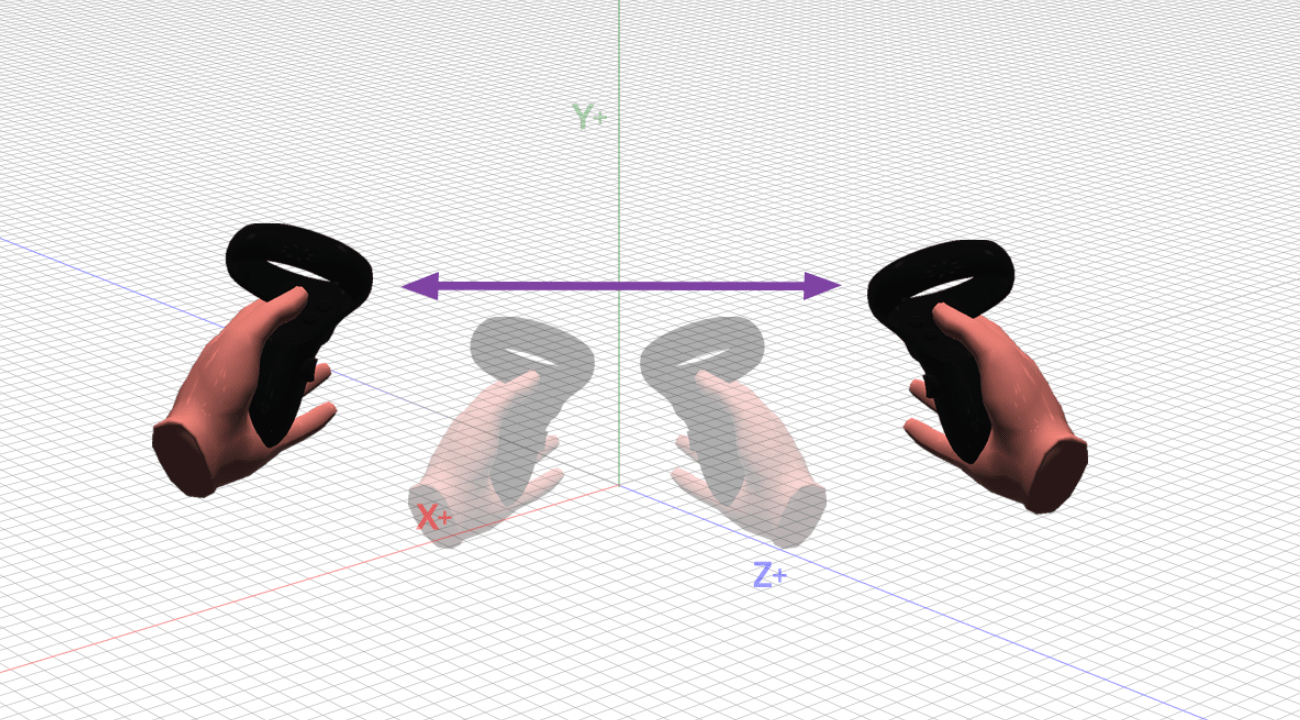
\includegraphics[width=\textwidth]{scaling}
    \caption{Zooming in the network functionality. The user can hold the scaling buttons on the Oculus controller to make the network bigger or smaller. In this example, if we stretch our hands outside, the network will expand.}
    \label{fig:scaling}
\end{figure}%


In Figure \ref{fig:scaling} there is a visual example of how the zooming works using the Oculus controllers. In this example, the user is stretching the hands out in order to make the network bigger. The user starts in an initial position, then holds the zooming triggers from both controllers, and then moves the hands out. If we wanted to make the network smaller we would do the opposite action, by contracting the hands to the inside.

\subsection{Interaction with the nodes}
GeneNet VR provides also information about the data that is being displayed. The user can interact with the nodes of the network to obtain information about each of them. In our example, the nodes represent genes and the user might be interested in knowing which gene name corresponds to a specific node. The action that we need to do to obtain the name of the gene is to get close with the right controller to the node that we are interested in and press the “5. Select node” index trigger on the right controller (see Figure \ref{fig:oculus_quest_inputs}). When we press this trigger, we can select a node from the network using a laser pointer. By selecting a node, we will get the name of that gene node that will be displayed in a rendered text, and we will also visualize the edges from this node to other nodes, represented with lines.

\subsection{Node relationships}
Finally, our dataset has information about the relationships between the nodes. GeneNet VR is implemented to show also this information. Because there can be too many relationships in the dataset, we don't show them all at the same time. Therefore, we can only see those of the node that the user has selected. The way that these relationships are represented is with lines between the nodes.


\section{Scalable network in Unity and data structures}
GeneNet VR uses files from an external source with data that will be used to be the network. The first file contains the information about the nodes and what category the node belongs to; The second one has information about the relationships between each of the nodes. As for the content of the files look like, in Table \ref{tab:categories-data} and Table \ref{tab:network-data} we show an extract from them. Originally the files are in CSV format. CSV \cite{csv} stands for Comma-Separated Values where each record is located on a separate line within the file, delimited by a line break. In addition, each record can contain one or more fields, separated by commas.

For our example, we represent the extract from the CSV files using tables, which are more illustrative. Table \ref{tab:categories-data} contains an extract from the file with information about the genes and the categories to which each gene belongs to. Here each row is a category and as we can see, the second cell contains all the gene names for that specific category. These categories are named by colors and these color names will be used by GeneNet VR to color each node from the network. As for the second table, Table \ref{tab:network-data}, this one shows an extract with the information about the relationships between the genes. This file can be very large since each row in the CSV file corresponds to a relationship between two genes and one gene can be related to multiple genes. For instance one of the CSV files that GeneNet VR uses to build the relationships contains almost 90k lines.

\begin{table}[h!]
\centering
\begin{tabular}{ll}
\hline
category & genes          \\
\hline
brown   & ARHGAP30 FERMT3 ARHGAP25 CD53 PLEK IRF8 DOCK2\\
cyan  & SAFB MOB3A RAB35 ABR ASCC2 CDC37 ANKFY1 GLTSCR1\\
darkgrey  & RAB40C ZNF213 ZNF263 PIGQ RHBDF1 RAB11FIP3\\
darkorange  & TCEB1 MRPL13 ENY2 MTERF3 UBE2W WDYHV1\\
\end{tabular}
\caption{Fragment of the dataset with the categories and the genes belonging to each category from the biopsy sample.}
\label{tab:categories-data}
\end{table}

\begin{table}[h!]
\centering
\begin{tabular}{llll}
\hline
source & target & weight            & id          \\
\hline
AAMP   & ARGLU1 & 0.102486209330144 & AAMP-ARGLU1 \\
ACADM  & FOXN2  & 0.107506881676173 & ACADM-FOXN2 \\
ACADM  & MBNL1  & 0.12269622045714  & ACADM-MBNL1 \\
ACADM  & PPM1B  & 0.103496640767895 & ACADM-PPM1B \\
\end{tabular}
\caption{Fragment of the dataset used to build the network relationships of the blood sample.}
\label{tab:network-data}
\end{table}

The following diagram shown in Figure \ref{fig:create_network} schematizes the steps that we follow to build the network in Unity. We start with the 2 CSV files described before, containing the data about the nodes and the relationships. We process these CSV files in order to store the data in data structures in GeneNet VR. During the process of storing this data we also apply a clustering algorithm that will set the correct position for each node in the network. After doing this we can easily access the information about the nodes, their position, color and to which nodes they are related to in order to draw the edges. Finally, the network is created using a particle system.

\begin{figure}[h!]
    \centering%
    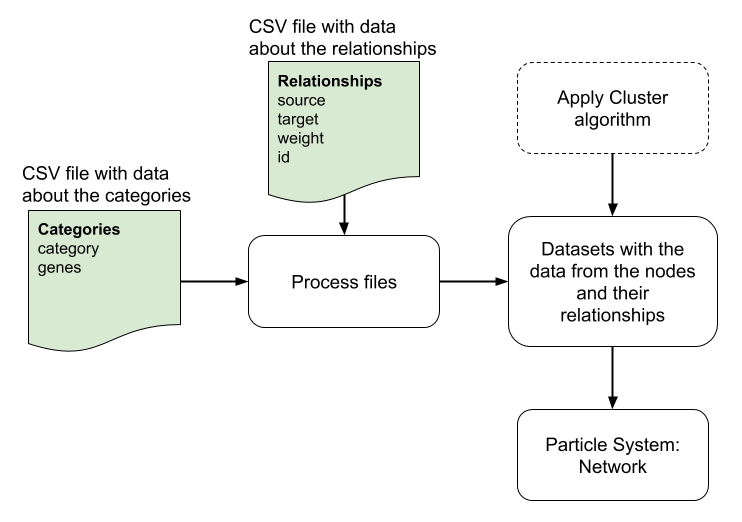
\includegraphics[width=\textwidth]{create_network}
    \caption{Diagram: steps for the creation of the network from the 2 CSV files.}
    \label{fig:create_network}
\end{figure}%

Now that we know how sources of information to build the network in GeneNet VR, let's take a look at how the network itself is represented in Unity and what algorithms and data structures we use for that. These will have an impact on the scalability of the network, and therefore it's important to choose a good solution. We have three elements from the network that have more weight in its scalability: the nodes, the edges, and the clustering algorithm used. We are going to explain each of them in more detail now.

The nodes in GeneNet VR are represented using a particle system. In Unity, a particle system \cite{particle_system} is defined as an array of particle objects. Each particle is a defined structure in Unity that contains properties like the life duration of the particle, start color, start size, or position in the 3D space. Particle systems in Unity are very useful to render some special effects like fire, steam, fireworks, or projectiles. They are also very powerful because they give plenty of control to the developer over the particles. In GeneNet VR we take advantage of this, allowing us to structure the network in the way we want. Usually, particles have a lifetime, which means that for instance they can start in a position with a particular color and finish or disappear after a few seconds in a different position and color. In GeneNet VR, the particles are static and have a very long lifetime, giving the perception that the network is a rigid structure. As for the way the particles are rendered, a 2-dimensional square is shown in the scene for each particle or node. Finally, in order to store the information of each node or particle we have a dictionary object in GeneNet VR that looks like this:

\begin{verbatim}
private Dictionary<string, ParticleSystem.Particle> particles;
\end{verbatim}

A dictionary in C\# is a data structure that contains a set of keys and each key has a single associated value. In our case, the key corresponds to the name of the node, the name of the genes in this case, and the value is a particle object.

The edges between the nodes are represented with 2-dimensional lines in GeneNet VR. A line in Unity is created with a Line Render component \cite{line_render}. These lines are very flexible and can be used to draw anything from a straight line to a spiral. They also have properties like color, texture mode, the possibility to have different widths along the line, etc. In our case we want to render straight lines, so we need to know the start and the endpoints where the line will be rendered. This information is taken from the CSV file with the edges' information. To store this information, we also use a Dictionary, where the key is the name of a node and the value is a list with all the nodes to which this node is connected to. This looks like this in C\#:

\begin{verbatim}
private Dictionary<string, List<string>> edges;
\end{verbatim}

Showing all the edges at the same time in GeneNet VR would make it very hard to visualize the network. For this reason, we show only the edges of the node that the user has selected. Also, in GeneNet VR the edges are shown dynamically, meaning that they are created every time the user selects a node. When the user selects a different node, the current edges are removed and a new set of edges are rendered for the new node. Every time an edge has to be rendered an edge object is instantiated with the CreateInstance method from Unity. The edge object in the scene from what is called a prefab in Unity. A prefab \cite{prefab} is basically a reusable asset, which in our cause is the line with some defines properties like the width and the color.

The algorithm used to cluster the nodes in the network is another important aspect that can influence the scalability. In GeneNet VR we use a linear algorithm that clusters the nodes in the 3d space depending on the module where they belong too. In this way, the user can visualize each module as single clusters with a distinct color per cluster.

\section{Other features of GeneNet VR}
GeneNet VR provides some features that help in the process of visualization and interaction with the network. We built a filtering system that allows the user to filter the nodes by using an interactive 2-dimensional menu. We also built a morphing feature that allows the user to compare two datasets in real-time, which can also be used on the 2-dimensional menu.

\subsection{Filtering information in the network}
Another feature that GeneNet VR uses to improve the visualization of networks is a filtering menu. When we have huge amounts of data in large networks, it is sometimes necessary to show less or more data. By filtering the nodes we can visualize only the part that we are interested in.

\begin{figure}[h!]
    \centering%
    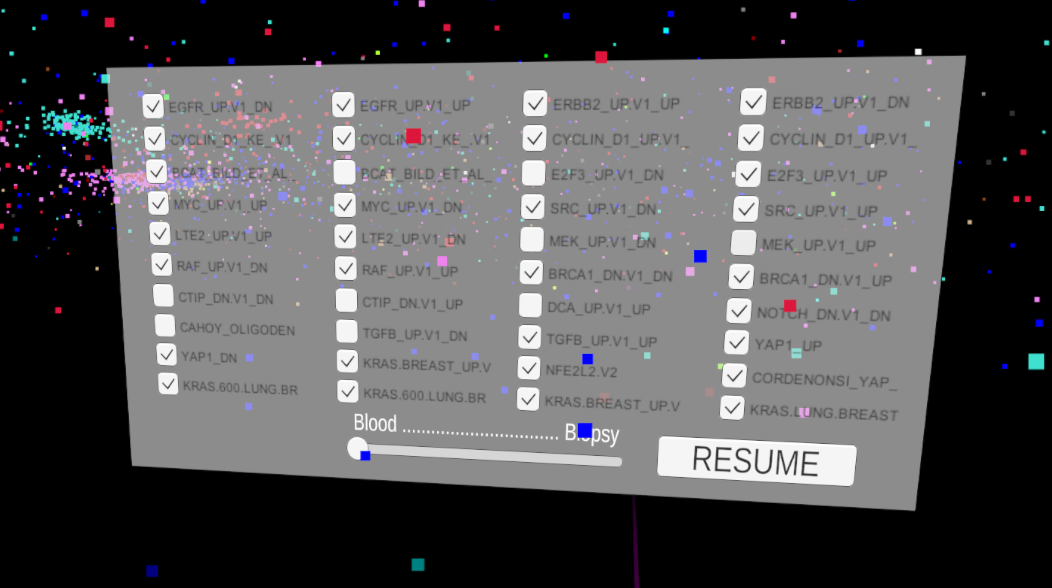
\includegraphics[width=\textwidth]{filtering}
    \caption{Filtering menu in GeneNet VR.}
    \label{fig:filtering}
\end{figure}%

We have built a 2-dimensional menu in Unity, see Figure \ref{fig:filtering}, to filter the data in our example network. We use checkboxes for filtering. From a starting point, all the boxes are checked, and if the user wants to hide apart from the visualization it is done by unchecking the box. To show the filtering menu we need to press the menu button from the left controller, see the “2. Filter menu” in Figure \ref{fig:oculus_quest_inputs}. To check or uncheck the boxes we need to use the A button from the right controller, named “6. Select item”, see Figure \ref{fig:oculus_quest_inputs}.

\subsection{Network morphing}
GeneNet VR has also the possibility to morph from one network to another. This can be done in the filtering menu by pressing the menu button from the left controller and there we can see a slider as in Figure \ref{fig:filtering} which we can move to the right or to the left in order to morph the network. In Figure \ref{fig:morphing} we can see an example of how the network morphs, showing 4 states of the morphing process. In a) the network is showing the blood network state and on d) the biopsy state. In b), the slider is moved slightly to the right, but closer to the blood state. We can see that in this state, the biopsy network is starting to show. Also, some nodes from the blood network are starting to move to relocate to their position in the biopsy network. In c) the slider is set closer to the biopsy state (to the right extreme) and we can appreciate more clearly the biopsy dataset, but the blood one is less visible.

This morphing tool helps us visualize two datasets at the same time and compare them. The slider has values from 0 to 10. When the value is set to 0 we visualize the blood dataset, and when it is set to 10, we visualize the biopsy dataset. For the values that are neither 0 nor 10, we can see both datasets at the same time. Depending on if the value is closer to 0 or 10, the nodes from one dataset or the other will be more visible. In addition, the position of the nodes that are found in both datasets is interpolated, and therefore we can see how these nodes move from one dataset to the other one by using the slider. Something that this tool doesn't allow us to do, is the selection of nodes and edges to render. We can only select the nodes if we are in either the blood or the biopsy state.

\begin{figure}[h!]
    \centering
    \begin{subfigure}{\textwidth}
      \begin{subfigure}[t]{0.5\textwidth}
          \centering
          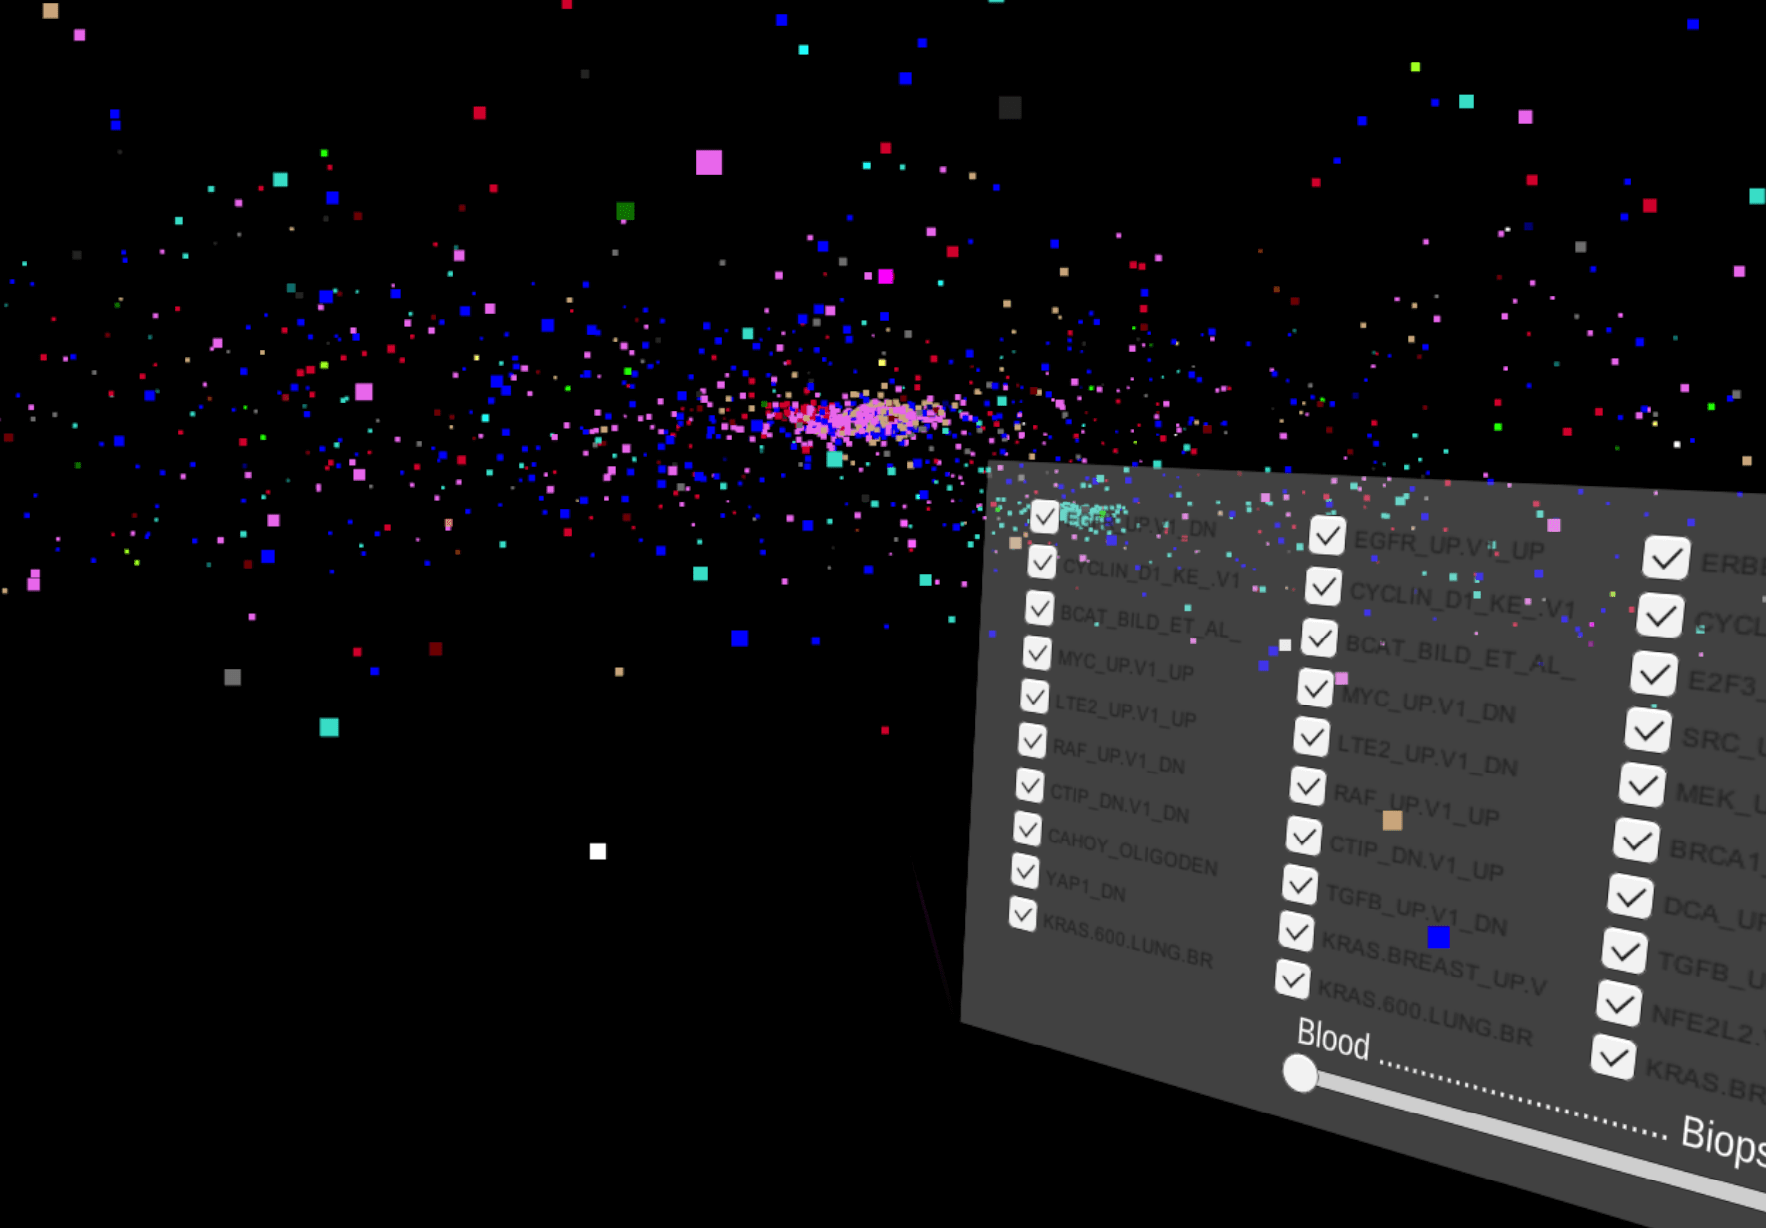
\includegraphics[width=\linewidth]{morphBlood}
          \caption{Slider set on the left extreme. It shows only the blood dataset.}
          \label{fig:morphBlood}
      \end{subfigure}
      \begin{subfigure}[t]{0.5\textwidth}
          \centering
          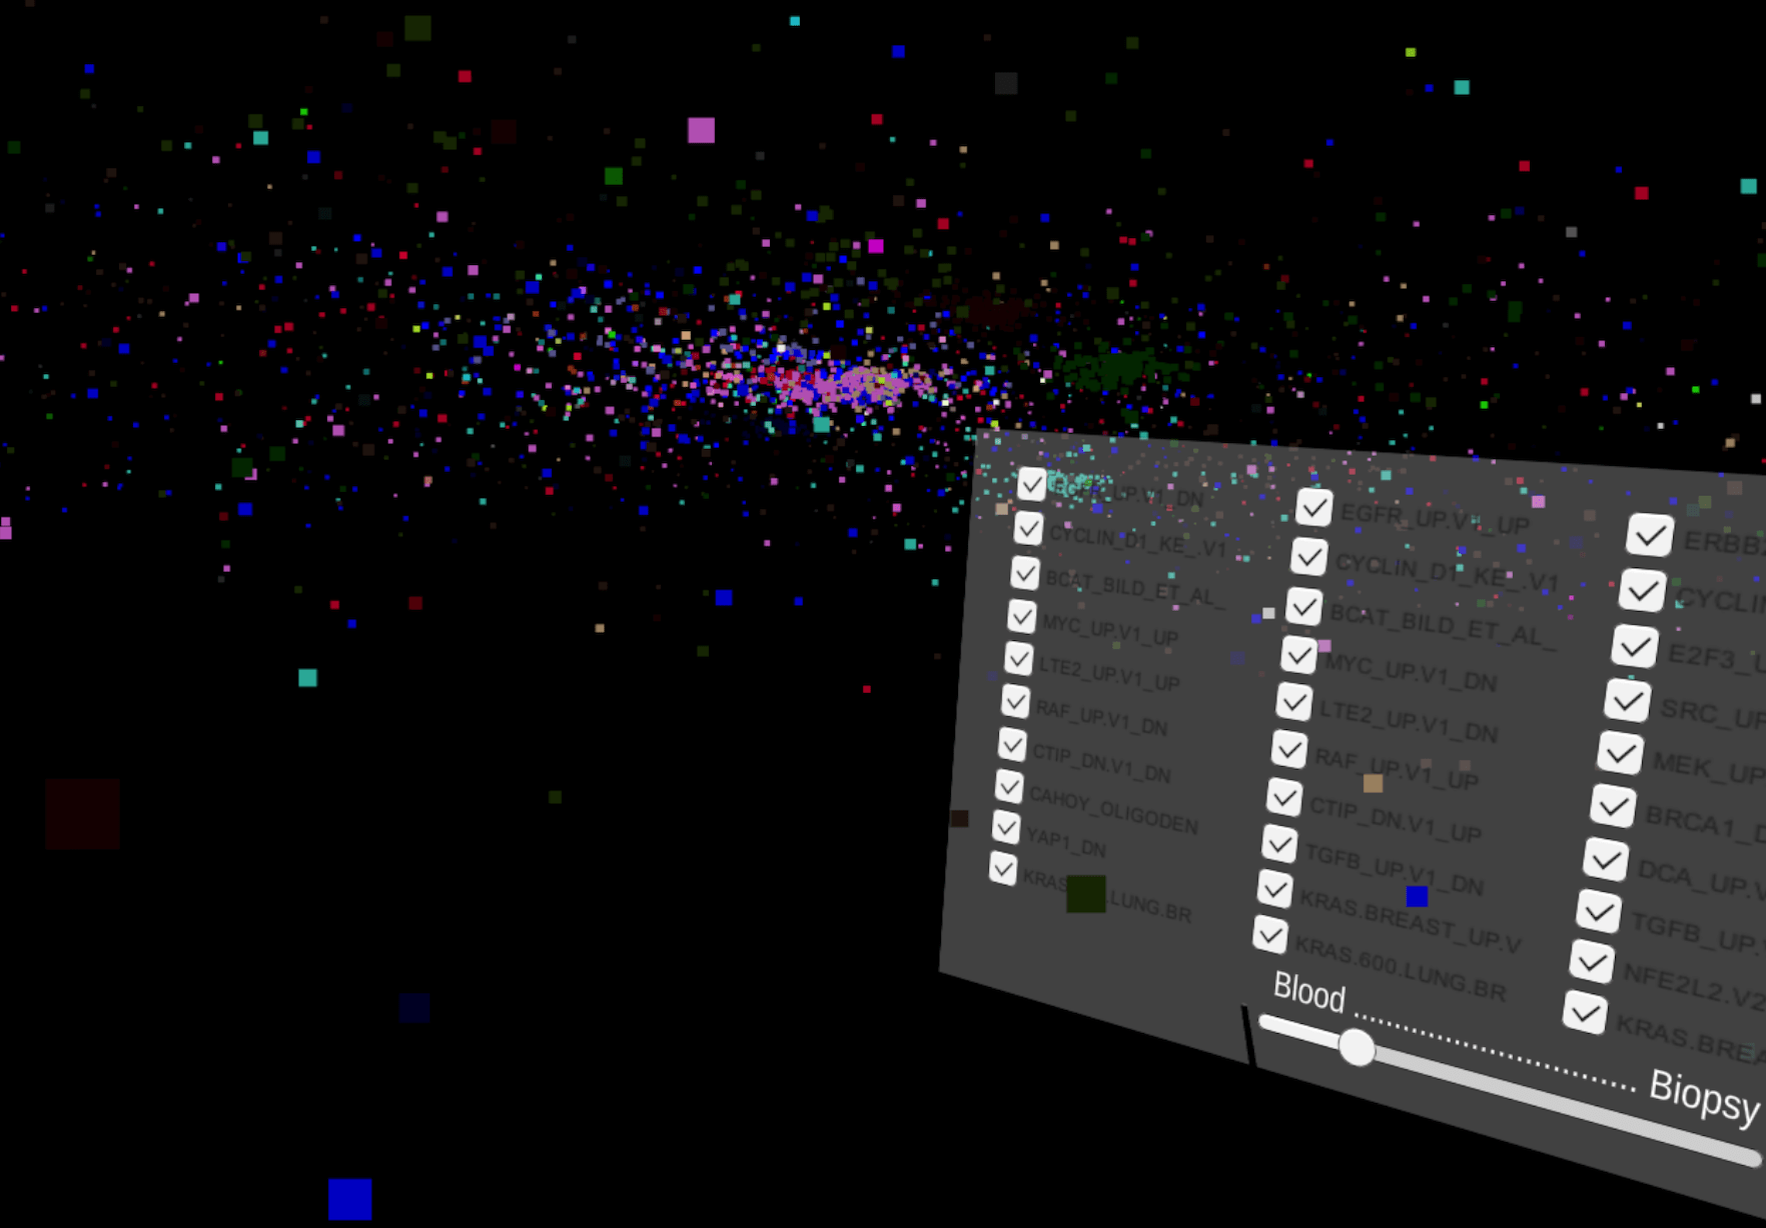
\includegraphics[width=\linewidth]{morph1}
          \caption{Slider set closer to the blood dataset. The biopsy dataset is more faded.}
          \label{fig:morph1}
      \end{subfigure}
    \end{subfigure}

    \begin{subfigure}{\textwidth}
      \begin{subfigure}[t]{0.5\textwidth}
          \centering
          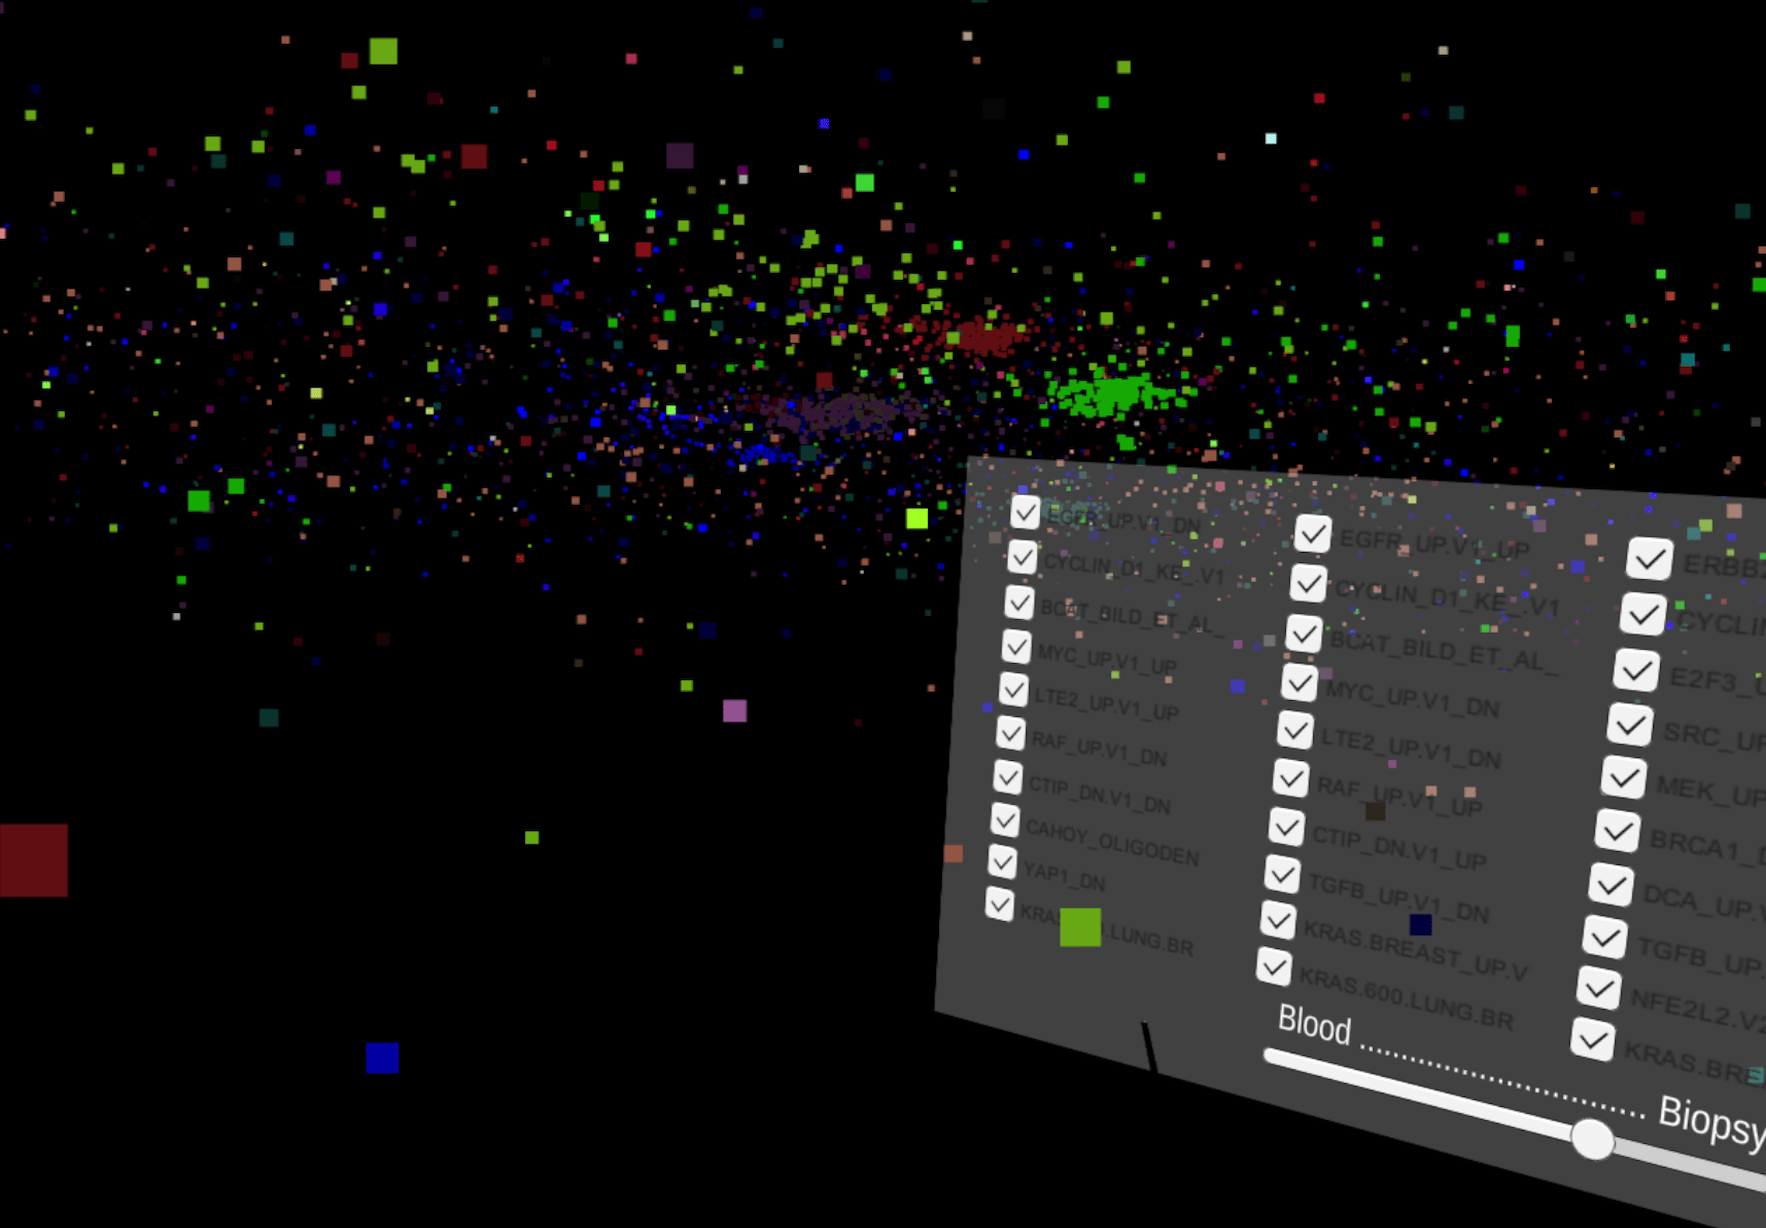
\includegraphics[width=\linewidth]{morph2}
          \caption{Slider set closer to the biopsy dataset. The blood dataset is more faded.}
          \label{fig:morph2}
      \end{subfigure}
      \begin{subfigure}[t]{0.5\textwidth}
          \centering
          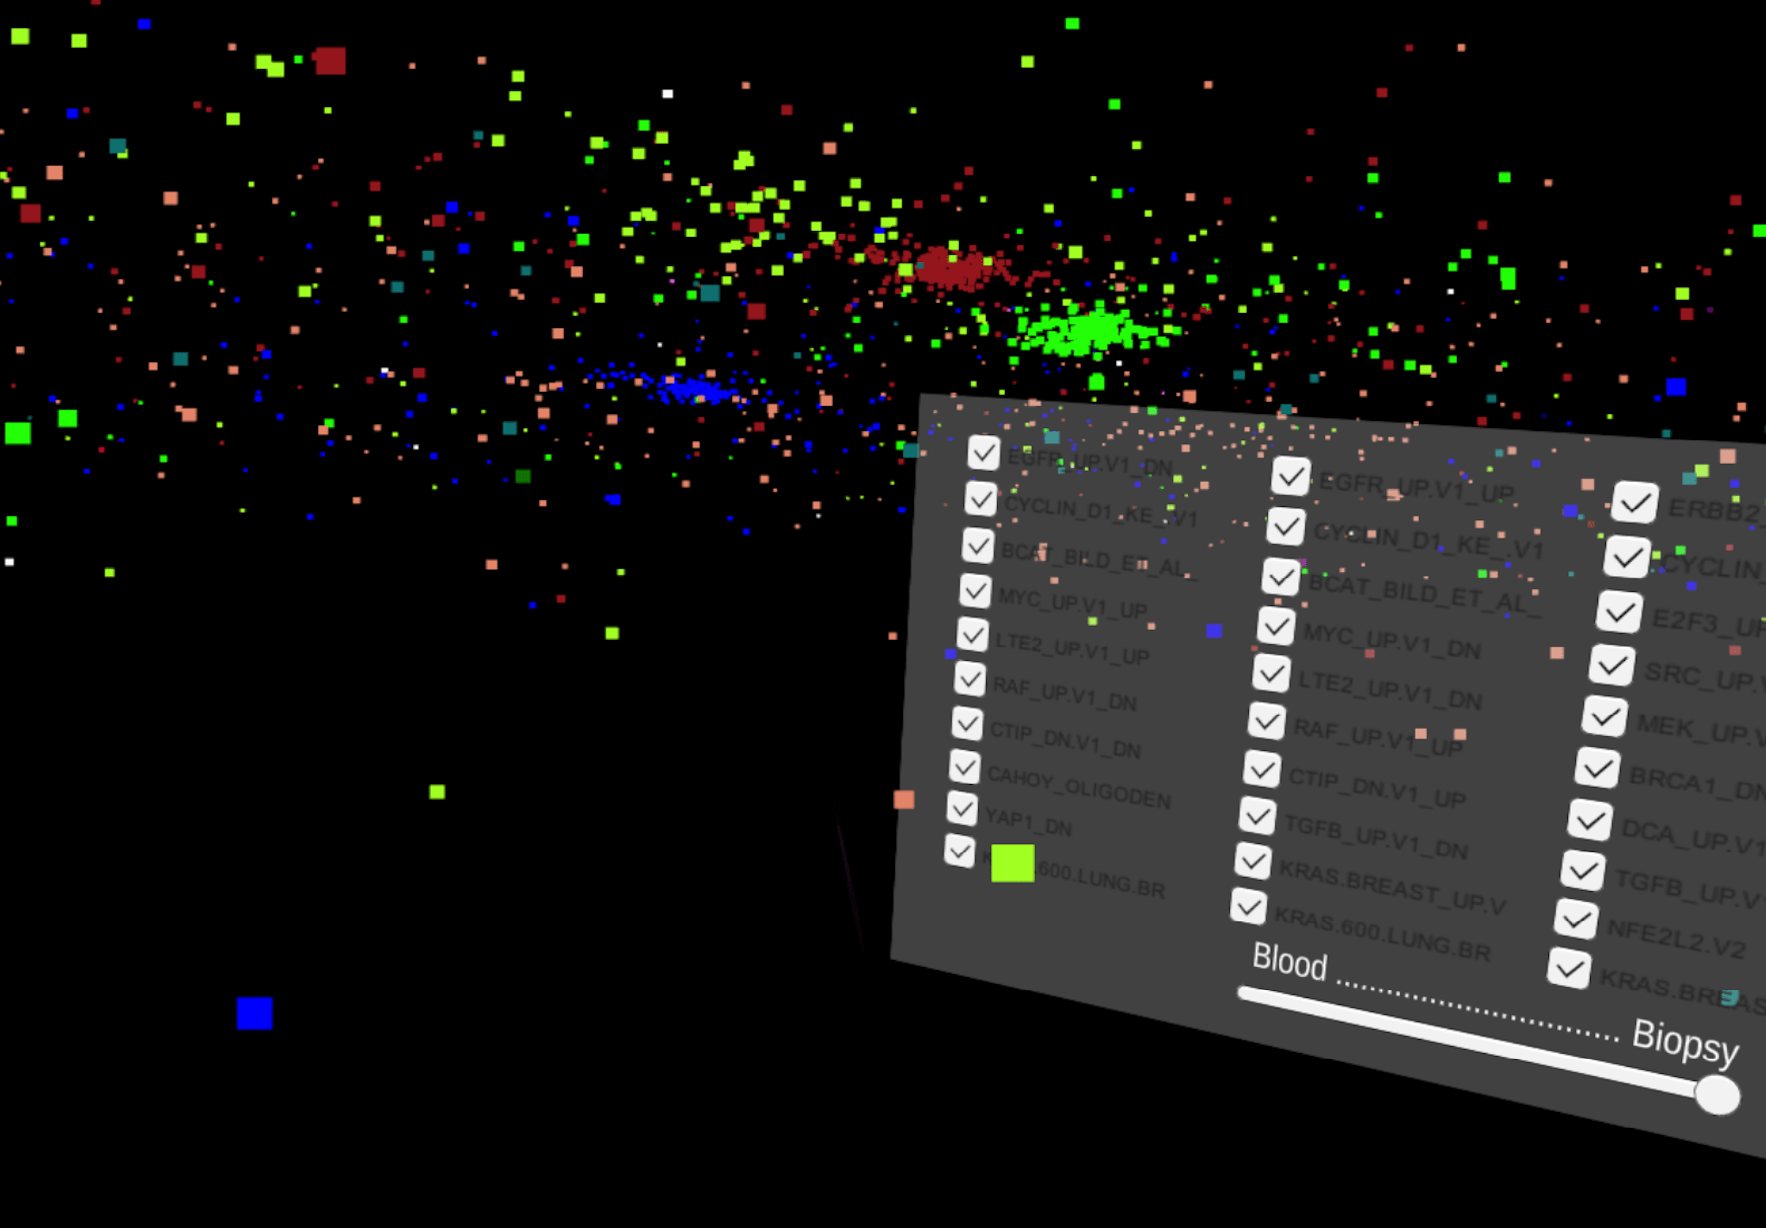
\includegraphics[width=\linewidth]{morphBiopsy}
          \caption{Slider set on the right extreme. It shows only the biopsy dataset.}
          \label{fig:morphbiopsy}
      \end{subfigure}
    \end{subfigure}

    \caption{Network morphing from the blood dataset to the biopsy dataset.}
    \label{fig:morphing}
\end{figure}

\section{Implementation details}
Unity (version 2018.4.10f1 \cite{unity2018}) is the software that was used to build the system. It is a multi-platform game engine. It is known to be easy to use and for having a big community of creators and asset designers \cite{developing_vr_unity}. Even though it is intuitive to use, it also has low-level access for developers. As for Virtual Reality, Unity has been up-to-date with the new VR technologies thanks to professionals and amateurs in this area who have built an integration for Unity. In our case, our device is an Oculus Quest, and for this reason, we use the Oculus integration for Unity \cite{oculus_unity_integration}. In addition, we have used VRTK, a collection of scripts and assets that help build VR solutions \cite{vrtk_what}. Finally, the programming language used in Unity to implement the system is C\#.

\section{Architecture and design}

\begin{figure}[h!]
    \centering%
    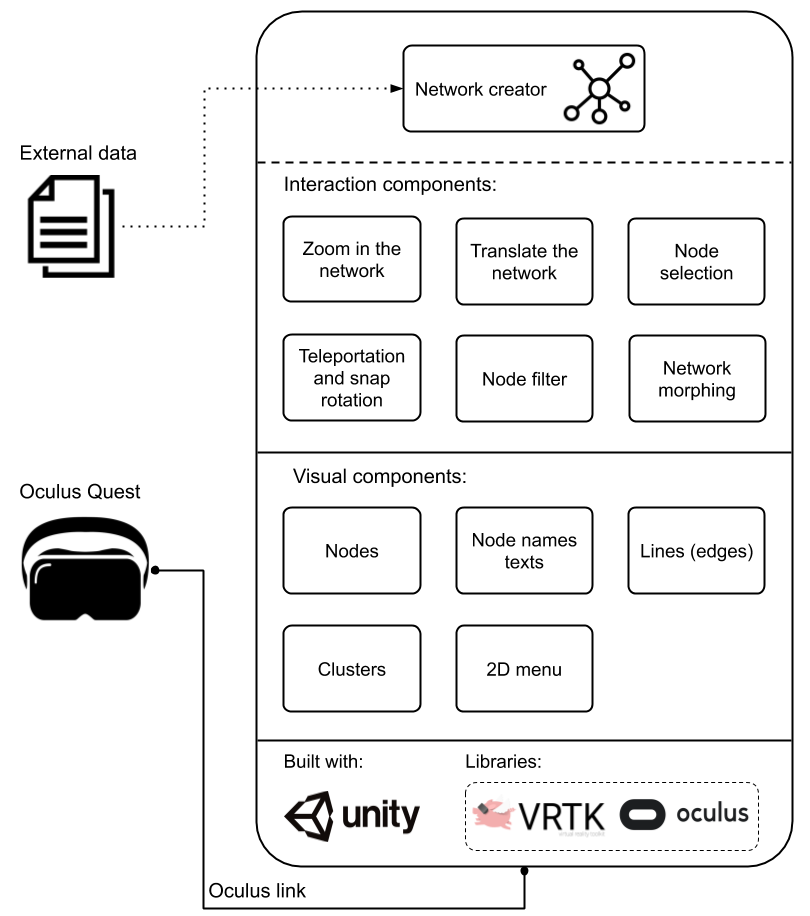
\includegraphics[width=\textwidth]{architecture_design}
    \caption{Architecture and design of GeneNet VR.}
    \label{fig:architecture_design}
\end{figure}%

GeneNet VR is a VR application built in Unity. For the implementation of the different visualization and interaction components, I programmed some C\# scripts, used also solutions that are native in Unity like the particle systems, and made use of the VRTK library and the Oculus library for Unity.

In Figure \ref{fig:architecture_design} we have an overview of the architecture of GeneNet VR. The big-box represents the Unity application and it contains all the components and functionalities that I have developed for the project. We can see that the big box is divided into 4 regions. The first one, starting from the top, is the network creator component that uses external data in order to build the network. In the second region, we have different interaction components that are available for the user to interact with the network and the environment. The third region contains the visual components that help the user visualize the data. Finally, the last region contains the technologies and libraries that I have used to build the application. We can also see the Oculus Quest headset represented down on the left. Here the user can visualize the network and use the controllers to interact. As we can see in the figure, the Oculus Quest can be connected to the PC using an Oculus Link, which is basically a high-quality USB 3 C to C or USB A to C cable with proven performance \cite{oculus_link}. This allows the user to run GeneNet VR on the PC. Another possibility is also to load GeneNet VR in the Oculus Quest and run it in the hardware of the headset without any cable or PC.

In this section, we will also mention some actions that are triggered using the Oculus controllers. These are specified in Figure \ref{fig:oculus_quest_inputs}.

\begin{figure}[h!]
    \centering%
    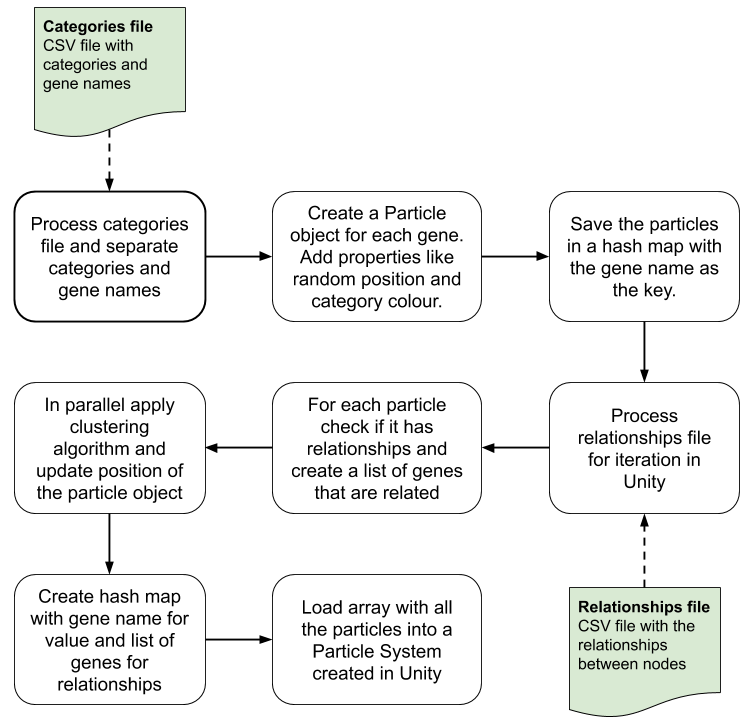
\includegraphics[width=\textwidth]{network_creator}
    \caption{Network creator algorithm.}
    \label{fig:network_creator}
\end{figure}%

The network creator (see Figure \ref{fig:network_creator}) initializes and builds the networks using the data files that were previously stored in the application's directory. It processes the data from the CSV files and stores the information in hash maps that can be later be used by the interaction components to transform or read the data of the networks like the node positions or colors. During this process of building the network, we apply a clustering algorithm as well. This algorithm consists of a loop of 10 iterations where for each iteration we go through each of the relationships from the relationship file. For each relationship we update the position of the nodes so that the ones that are connected are closer to each other in the space, resulting in clusters of nodes depending on how related they are.

For the \textit{zoom in the network} component I wrote a C\# script where I use the Oculus integration to communicate with the Oculus Quest controllers. The algorithm is run every time the user enables the action for zooming (see Figure \ref{fig:network_zoom} for the algorithm). What the script does is to find out if the user is stretching or contracting the arms. For this, when the user triggers the action, the system stores the current position of the left and right controllers in the 3D space and calculates the distance between these 2 points. This position is called initial position. Until the user releases the triggers, the system calculates for every frame the current distance between the two controllers and compares it with the initial distance that was stored right before the user triggered the action. If the new distance is smaller than the initial one, the network will shrink; if it is bigger, the network will grow up.

\begin{figure}[h!]
    \centering%
    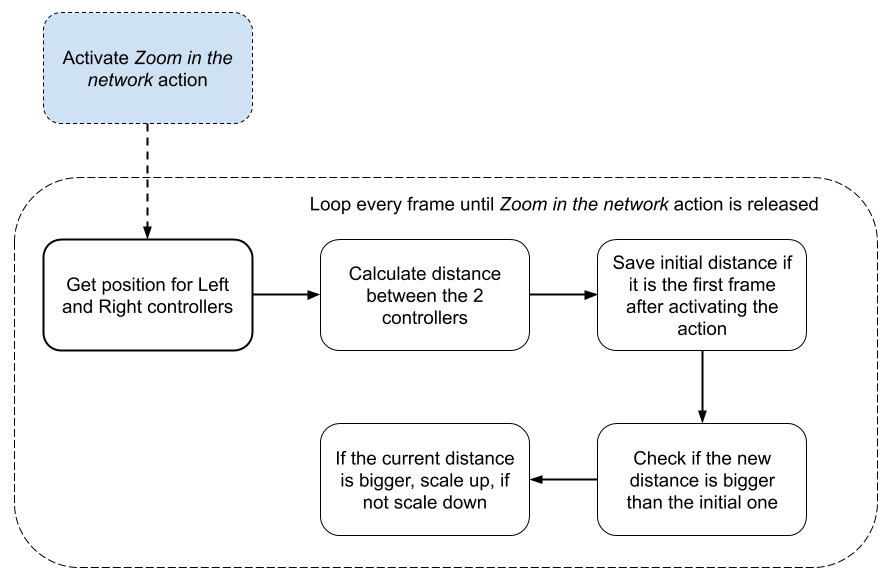
\includegraphics[width=\textwidth]{network_zoom}
    \caption{Algorithm for zooming in the network.}
    \label{fig:network_zoom}
\end{figure}%

The \textit{translate the network} component consists is implemented in C\# as well (see Figure \ref{fig:network_translator}). Here we do something similar to the \textit{zoom in the network} component. When the action for the translation of the network is triggered, the position of the right controller is stored as the initial position. Then, while the user is holding the trigger of the right controller, the current position for the controller is calculated for every frame. A vector is calculated as (current\_position - initial\_position) and normalized. With this we obtained the direction of the vector where the user is trying to move the network to. We add up that vector with a constant to update the position of the network in the 3D space.

\begin{figure}[h!]
    \centering%
    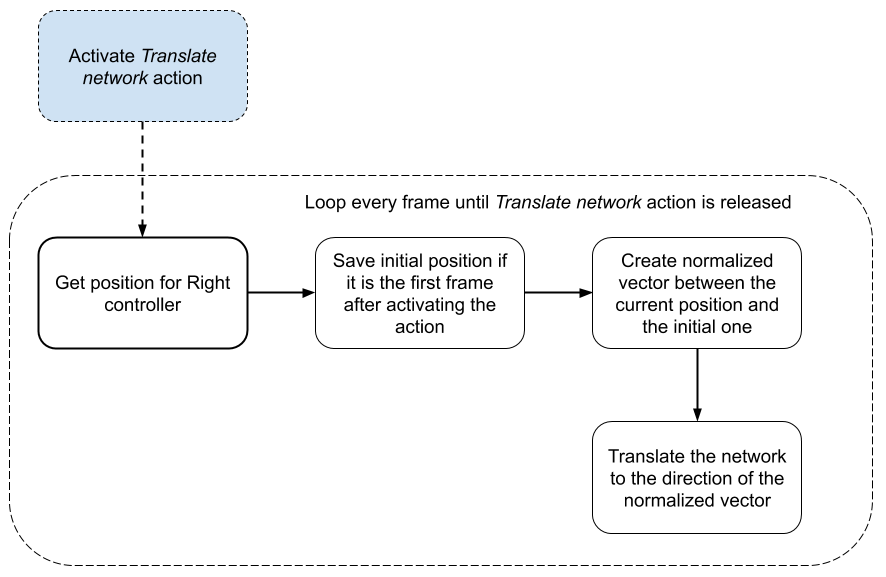
\includegraphics[width=\textwidth]{network_translator}
    \caption{Algorithm for translating the network.}
    \label{fig:network_translator}
\end{figure}%

For the \textit{select node} component, when the user triggers the \textit{select node} action, an algorithm is used to calculate which node is the one that the user is trying to point at. In Figure \ref{fig:select_node}, we can see a flowchart of the algorithm that we implemented. I used C\# to code a script for this functionality. A laser pointer comes out from the right controller when the user triggers the action. In the algorithm, we make use of this laser information which consists of a vector. In order to select the node that we are pointing at, we calculate for each node in the network a vector product composed of the laser vector and a vector that goes from the right controller position to each node position. The result is another vector where we extract its magnitude. The magnitude that is smaller will correspond with the node that is closer to the laser pointer. We will select this node with a smaller magnitude value. When a node is selected, the algorithm also draws the lines corresponding to the relationships of this node in the scene. If there were any lines before the new node is chosen, these are removed.
\begin{figure}[h!]
    \centering%
    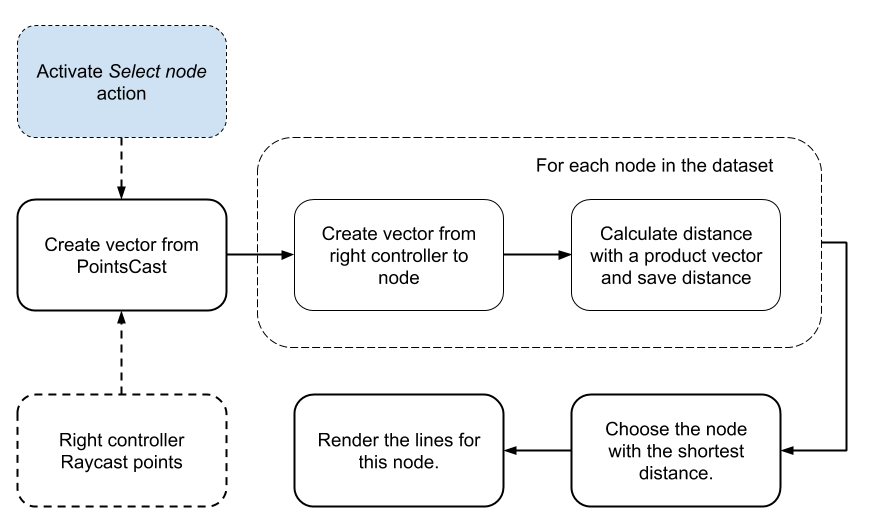
\includegraphics[width=\textwidth]{select_node}
    \caption{Algorithm for the selecton of the nodes in the scene.}
    \label{fig:select_node}
\end{figure}%

The \textit{network morph component} (see Figure \ref{fig:network_morph}) consists of a UI slider element that is in the menu and a method where we pass the value of the slider as a parameter. The values from the slider range from 0 to 10 and as the algorithm shows, value 0 will show the blood network in the scene and value 10 will show the biopsy one. When the value is greater than 0 or lower than 10, we interpolate the color and the position of the nodes. For the color interpolation, we use a linear interpolation function from Unity called Color.Lerp. The position interpolation is only applied to the nodes that are in both the blood and the biopsy dataset. For this interpolation, we create a vector that goes from the node in the blood dataset to the node in the biopsy one. We divide this vector into 10 and multiply it for the slider value. This will be the new position for the node.
\begin{figure}[h!]
    \centering%
    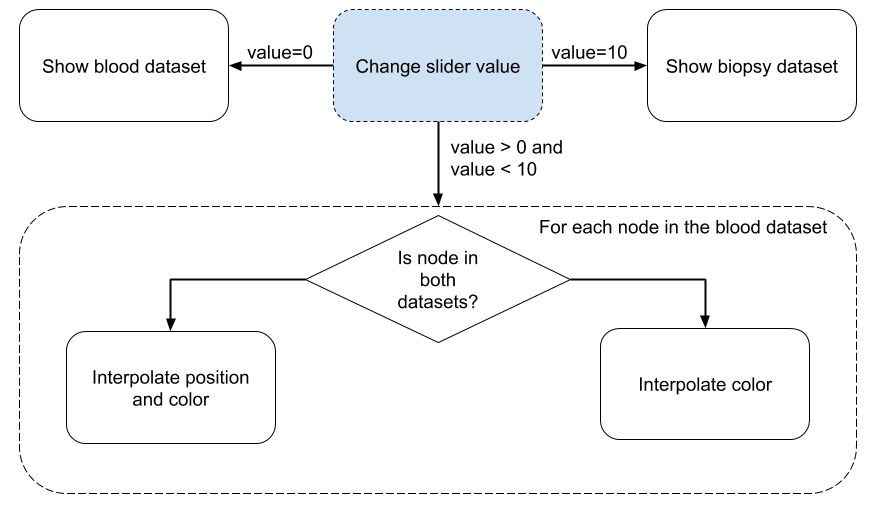
\includegraphics[width=\textwidth]{network_morph}
    \caption{Algorithm for the network morph.}
    \label{fig:network_morph}
\end{figure}%

For the \textit{node filter component}, a UI interface is used in Unity. This interface contains several checkboxes that are switched on by default. In addition, each checkbox has attached a function that is run every time the user switches it off or on. This function receives as a parameter a string value that is different from each checkbox. When the user switches  the checkbox, the algorithm looks into a hash map that looks like this:

\begin{verbatim}
private Dictionary<string, string[]> oncoGroups;
\end{verbatim}

We use the string variable that is passed to the function to look up the oncoGroups hash map, where each key corresponds to the name of each checkbox. We obtained a list of nodes that we need to turn on or off from the network.

Finally, for the \textit{Teleportation and snap rotation component} we have used some scripts and prefabs that come with the VRTK library. I used as a reference for some techniques to develop these locomotion solutions from a course on Unity\footnote{https://learn.unity.com/course/oculus-vr}.


\chapter{MIxT}
% What is MIxT used for? And how would users do it in VR?
% How the MIxT application is implemented in GeneNet VR and what it does.
% What are typical network characteristics for this (type of) application? Size, clusters, edges, connectivity, etc?

The Matched Interaction Across Tissues (MIxT) is a system developed by UiT and Concordia University for exploring and comparing transcriptional profiles from two or more matched tissues across individuals \cite{fjukstad_dumeaux_olsen_lund_hallett_bongo_2017}. This system is implemented as a web application and it has a 2-dimensional visualization tool to explore biological networks \footnote{https://mixt-tumor-stroma.bci.mcgill.ca/network}. This tool has, however, some known scalability and visualization problems.

We have used MIxT in GeneNet VR as a case study. In addition, we used this case study in the evaluation since it is a realistic application where we used complex networks that originally didn't scale in the existing web application. In this chapter we will describe what MIxT is used for, its disadvantages for scaling large biological networks and the challenges of building a VR visualization system that can solve the visualization and scalability problems.

\section{What is MIxT used for?}
MIxT is a web application for interactive data exploration in system biology developed by UiT and Concordia University. A reasearch was carried out for the study of interactions between the tumor and the blood systemic response of breast cancer patients. In the study, they profiled RNA in blood and matched tumor from 173 patients with breast cancer. The goal of the study was to identify genes and pathways in the primary tumor that are tightly linked to genes and pathways in the patient's systemic response (SR). The SR is the body's response to an infectious or non infectious insult. A biological pathway is a series of actions among the molecules in a cell that leads to a certain product or change in the cell. The result of the study suggests new ways of monitor breast cancer by looking outside the tumor and studying the patient's systemic response.

MIxT provides an interactive view for networks. In Figure \ref{fig:mixt_webapp}, we show a screenshot from the network view. This view is two-dimensional and the user can do some interactions to explore data, but these are very limited. The users can zoom in and zoom out and also drag and drop with the mouse in the view in order to "move around". Also, by hovering on a node, the user can see the name of that node. By clicking on a node, the user goes to another page with more detailed biological information about that gene.

\begin{figure}[h!]
    \setlength{\tempheight}{15ex}
    \centering
    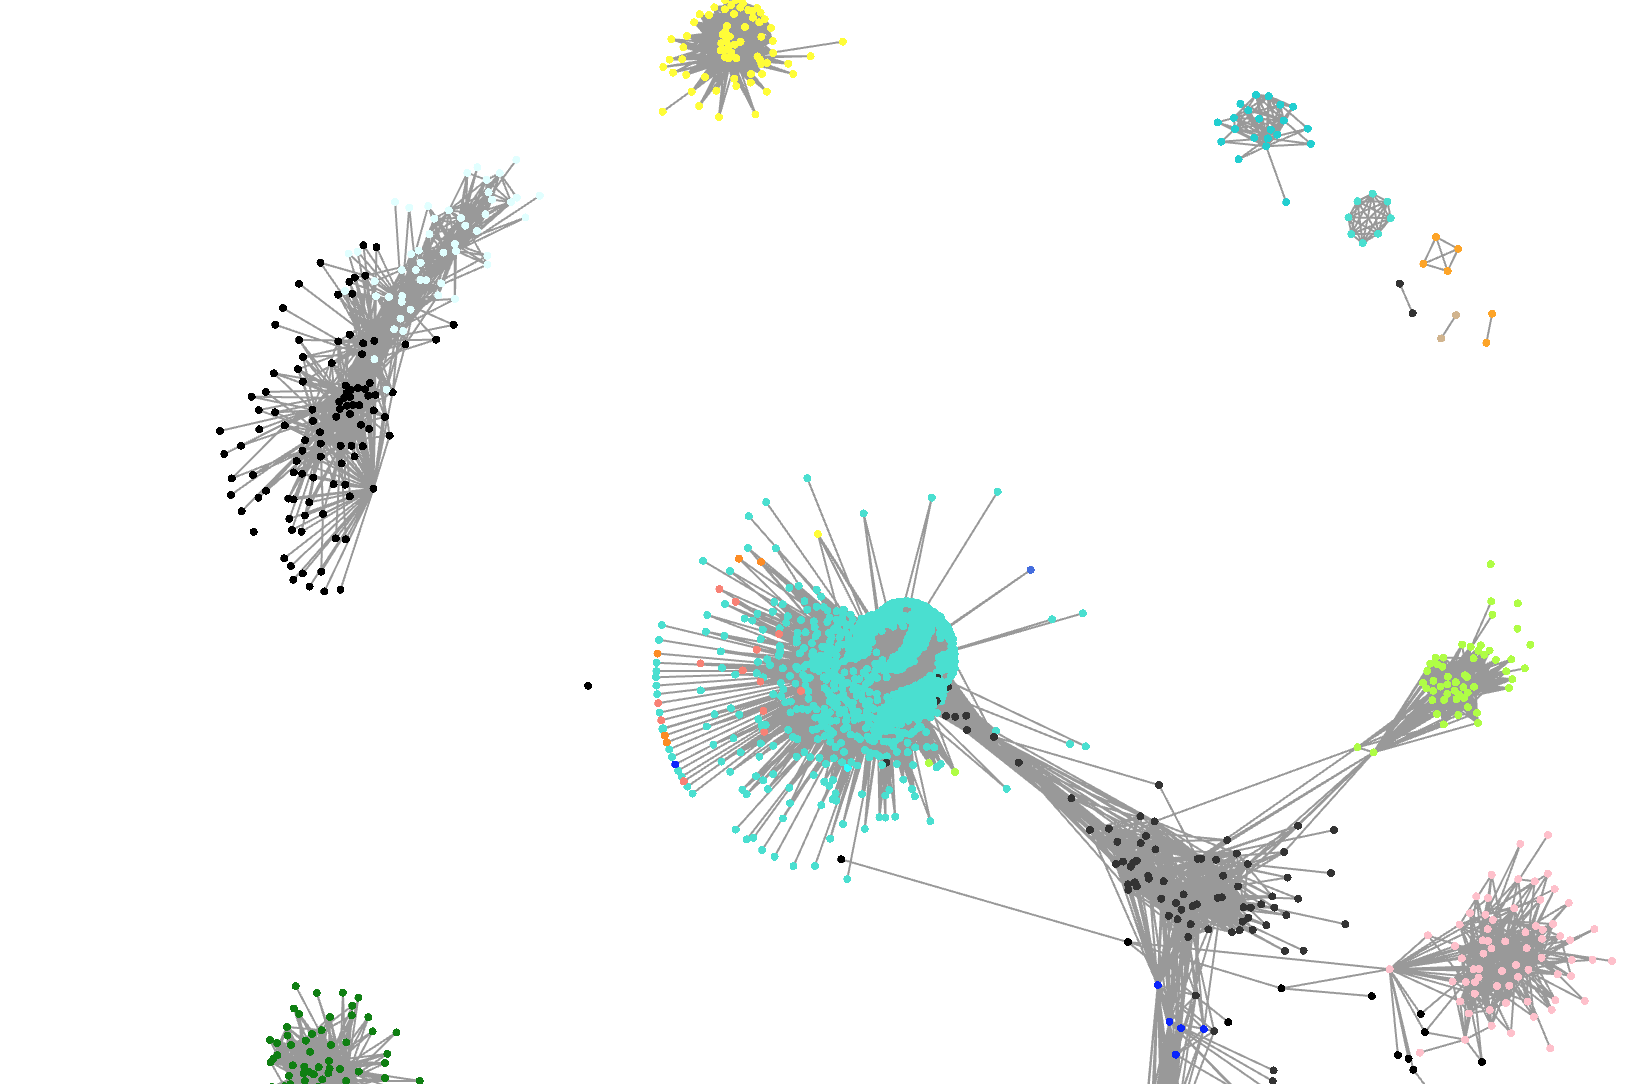
\includegraphics[width=\textwidth]{mixt_webapp}
    \caption{Screenshot from the network view in the MIxT web application.}
    \label{fig:mixt_webapp}
\end{figure}

An evident problem in this view appears when we start to explore the network. The clusters have many nodes and each node can have multiple edges, so the graph ends up looking like a hairball and it is not easy to explore (see Figure \ref{fig:mixt_hairball} for a screenshot of this problem from MIxT). In addition, the edges need to be rendered every time the user interacts with the network. It may take a few secons until the user can view all the edges that are in the view frame. This is a problem since the user needs to do many interactions when exploring the network. The visualization process becomes cumbersome and tedious in MIxT.

\begin{figure}[h!]
    \setlength{\tempheight}{15ex}
    \centering
    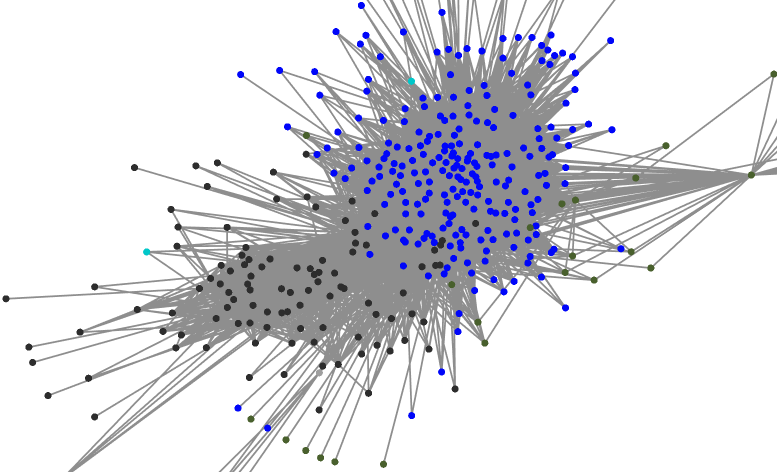
\includegraphics[width=\textwidth]{mixt_hairball}
    \caption{Hairball problem in the network view in MIxT.}
    \label{fig:mixt_hairball}
\end{figure}

\section{MIxT in VR}
We have implemented a Virtual Reality version of the network view from MIxT in order to solve some scalability and visualization problems that this tool has. In addition to the originally challenges that the network visualizer has, there other challenges that we need to take into account in VR. In this section, we are going to explain these challenges and how we solved them in GeneNet VR.

When moving the original visualization system to VR, we have to count with a new dimension and also the immersive feeling for the user. Having a new dimension is an advantage when we want to visualize high-dimensional data, like gene networks. However, we need to cope with occlusion problems. When the user visualizes the network from a particular angle, the nodes and edges that are in front of the user's viewpoint may hide other nodes and edges that are behind them. To solve this problem, we need to give the user the possibility to view the network from different angles. In GeneNet VR we have implemented a locomotion solution that allows the user to teleport to other parts of the scene. The user can also rotate the viewpoint to the right or to the left. In addition, the user has the possibility to move the network around by using the VR right controller.

As we mentioned before, the original network view from MIxT has an information overload problem. The network looks like a hairball and it's hard to explore it and find patterns in it. To solve this problem in VR, we show only the edges from the nodes that the user wants to explore. This solution reduces the amount of information that is shown, but it needs some interaction solutions so that the user can easily explore the edges of the network. In GeneNet VR, we have implemented a node selector that allows the user to select a particular node using a laser pointer. When the laser collides with a node, the edges of this node are shown. Also, the user can scale up and down the network by using the VR controllers. In addition, a filtering menu was implemented in GeneNet VR, where the user can filter out the information from the network that is not relevant.

Another problem from the MIxT network view is that it can be slow when visualizing the data. The nodes may take a few seconds to show completely, so the visualization process can be hard.

\section{Network characteristics}
The human being has 23 pairs of chromosomes in each of our cells. Each chromosome can contain from hundreds to thousands of genes. There are estimated to be around 30.000 genes. In GeneNet VR, the blood dataset is the biggest one, and contains a total of 2693 genes. We don't expect to deal with a network of 30.000, but it is true, as we can see from the datasets, that they can contain several thousands nodes and also several thousand edges. For instance, in the blood dataset, we can find a node that has 1607 relationships to other nodes.

[What are typical network characteristics for this (type of) application? Size, clusters, edges, connectivity, etc?]


\chapter{Evaluation and discussion}
% Benchmarking in Unity
% https://blogs.unity3d.com/2018/09/25/performance-benchmarking-in-unity-how-to-get-started/
% Maybe try VRWorks https://developer.nvidia.com/vrworks

% Questions to answer in the evaluation chapter:
% \begin{enumerate}
%   \item{How big can the graph be so that it is comfortable visualizing the network?}\\
%   What is comfortable? Number of FPS?
%   How can we scale the graph? By adding nodes and spread them around, by adding more interconnexions?
%   Should the experiment split in several parts? Scaling, filtering, moving around, etc.
%   What is the performance by using Oculus Link and the performance using just the Quest hardware?
%   -We can use the Unity GPU Profiler for Oculus Quest and Go in order to see the performance.\\
%   \href{https://developer.oculus.com/blog/getting-started-w-the-unity-gpu-profiler-for-oculus-quest-and-go/}{See: Getting Started w/ The Unity GPU Profiler for Oculus Quest and Go}
%   \item{How is this way of visualizing the graph better by using VR?}\\
%   We are researchging the technology and the test with actual users is for future work.
%   \item{In what way can the application and the visualization of the graph be improved?}\\
%   Argue in the discussion part.
% \end{enumerate}

% Links
% Profiler panel

BigNet VR has been implemented to explore biological networks like the one from MIxT. In this chapter we will evaluate the scalability of the application for this type of networks. The following list shows the questions that were asked as part of the evaluation and that we will try to answer along this chapter:
\begin{enumerate}
  \item How big can the biological network be so that it is comfortable to explore and visualize it?
  \item How can we scale the network?
  \item What is the performance by using Oculus Link and the performance using just the Quest hardware?
  \item How comfortable is it to explore a network?
\end{enumerate}

\section{Experimental setup}
% @TODO Write about the specs of the system being used for the evaluation: the machine, software, etc.
We ran the experiments in a machine with Windows 10 and the following hardware specification:
\begin{itemize}
  \item Processor: Intel(R) Xeon(R) CPU E3-1275 v6 @ 2.80GHz 3.79 GHz.
  \item RAM memory: 64.0 GB.
  \item System type: 64-bit Operating System.
\end{itemize}

GPU specifications:
\begin{itemize}
  \item Adapter type: NVIDIA GeForce GTX 1080 Ti.
  \item Chip Type: GeForce GTX 1080 Ti.
  \item DAC Type: Integrated RAMDAC.
  \item Total Available Graphics Memory: 45025 MB.
\end{itemize}

% @TODO Write about Oculus quest hardware
Oculus Quest specifications
\begin{itemize}
  \item Panel Type: Dual OLED 1600x1440.
  \item Supported Refresh Rate: 72Hz.
  \item Tracking: Inside out, 6DOF.
  \item CPU: Qualcomm® Snapdragon 835.
  \item GPU: Qualcomm® Adreno™ 540 GPU.
  \item Memory: 4GB total.
\end{itemize}

\section{Performance of the system}
% @TODO Write about how scalability was tested.
A test scene was built in order to test the network and the scalability of it. A random network is built and we test how comfortable it is to navigate through it. This is measured by the FPS rate.

VR profiling is a technique used to get an overview of the performance of our application. This is usually done in order to find bottlenecks so that we can eliminate them and improve the application's performance.

According to Oculus' performance baselines\cite{oculus_performance_baselines}, an application should meet the following requirements:
\begin{itemize}
  \item 72 FPS for Oculus Quest (required by Oculus).
  \item 50-100 draw calls per frame.
  \item 50,000-100,000 triangles or vertices per frame.
\end{itemize}

To profile the application we used the built-in profiler in Unity, the software used for the development. The Unity Profiler gives information about per-fram CPU and GPU performance metrics.

\section{Scalability of the system}

\section{Questionnaire to evaluate the system}
One of the questions that we asked ourselves during the evaluation process was about the comfortability of using BigNext VR to explore a biological network. This is an important aspect when building VR applications. Some of the aspects to take into account are for instance the motion sickness or the intuitiveness. In order to evaluate this we made a questionnaire for bioinformaticians that would test the application. Unfortunately, due to the Covid-19 situtation\cite{covid_19}, we were not able to run this testing process because it was not possible to have people testing the application on a single Oculus Quest device without avoiding the social distancing rules.
We estimated to have tested the project with at least 10 participants with knowdledge in bioinformatics. With this number of participants we can make some statistics. The questions that we prepared for the questionnaire were the following:\\

Indicate the level of agreement or disagreement with each of the following statements or just mark yes or no:
\begin{enumerate}
  \item Have you ever used a VR headset before?\\
  Yes / No

  \item I feel comfortable using the Oculus Quest headset.\\
  Strongly agree / Agree / Neutral / Disagree / Strongly Disagree

  \item I feel comfortable moving around the virtual environment using the teleport functionality.\\
  Strongly agree / Agree / Neutral / Disagree / Strongly Disagree

  \item I feel comfortable rotating to any direction.\\
  Strongly agree / Agree / Neutral / Disagree / Strongly Disagree

  \item I feel comfortable visualizing the network by moving my head.\\
  Strongly agree / Agree / Neutral / Disagree / Strongly Disagree

  \item I feel comfortable selecting the nodes to visualize the relationships.\\
  Strongly agree / Agree / Neutral / Disagree / Strongly Disagree

  \item I feel comfortable moving the network to the position that I want.\\
  Strongly agree / Agree / Neutral / Disagree / Strongly Disagree

  \item I feel comfortable scaling the network.\\
  Strongly agree / Agree / Neutral / Disagree / Strongly Disagree

  \item I feel comfortable opening the UI menu to filter the data from the network.\\
  Strongly agree / Agree / Neutral / Disagree / Strongly Disagree

  \item It is intuitive to manipulate the network using the controllers.\\
  Strongly agree / Agree / Neutral / Disagree / Strongly Disagree

  \item The different actions in the controllers are easy to learn and remember.\\
  Strongly agree / Agree / Neutral / Disagree / Strongly Disagree

  \item I can move the network to any position that I want.\\
  Strongly agree / Agree / Neutral / Disagree / Strongly Disagree

  \item I can scale the network to any size that I want.\\
  Strongly agree / Agree / Neutral / Disagree / Strongly Disagree

  \item I can select any node that I want.\\
  Strongly agree / Agree / Neutral / Disagree / Strongly Disagree

  \item I can easily visualize the relationships of any node.\\
  Strongly agree / Agree / Neutral / Disagree / Strongly Disagree

  \item I can easily filter the data in the network that I want to visualize.\\
  Strongly agree / Agree / Neutral / Disagree / Strongly Disagree
\end{enumerate}


\chapter{Related work}
I will focuse in this chapter on VR applications found in the literature for the visualization of bioinformatic data.

\section{Virtual Reality Chemical Space}
Virtual Reality Chemical Space is a VR application for the interactive exploartion of chemical space populated by Drugbank compounds\cite{drugbank}. It is also developed in Unity using C\# and the VRTK library. They use a particle system to render the particles of the chemical space. To render the particles, they use shaders instead of geometrical spheres as well, optimizing the number of vertices per datapoint in the scene. In order to reduce the motion sickness they have introduced a floor in the form of a grid acting as a static frame of reference. Also instead of letting the user move through the VR environment, they use a controller to move the point cloud. In Figure \ref{fig:drugbank} we can see an screenshot from the VR application. As we can notice in the screenshot, there is a subtle rendering of an outer space scene as an independent visual background. This is another technique to reduce the motion sickness that helps the user keep the notion of space. This is an interesting technique that we could have tried in BigNet VR.

They conclude in the article that the application that they have developed doesn't visualize an environment with an analogue in the real world, but instead a mathematical construct. Also some of the drawbacks that VR has compared to traditional solutions is that the VR headsets are not so comfortable as well as often-occurring eye strain and virtual reality sickness. They also conlcude that the application of VR in chemistry has more potential in the fields of education and training as for the current state of technology. The tools for chemistry need to be further evaluated wether they should be extended to VR.

\begin{figure}[h!]
    \centering%
    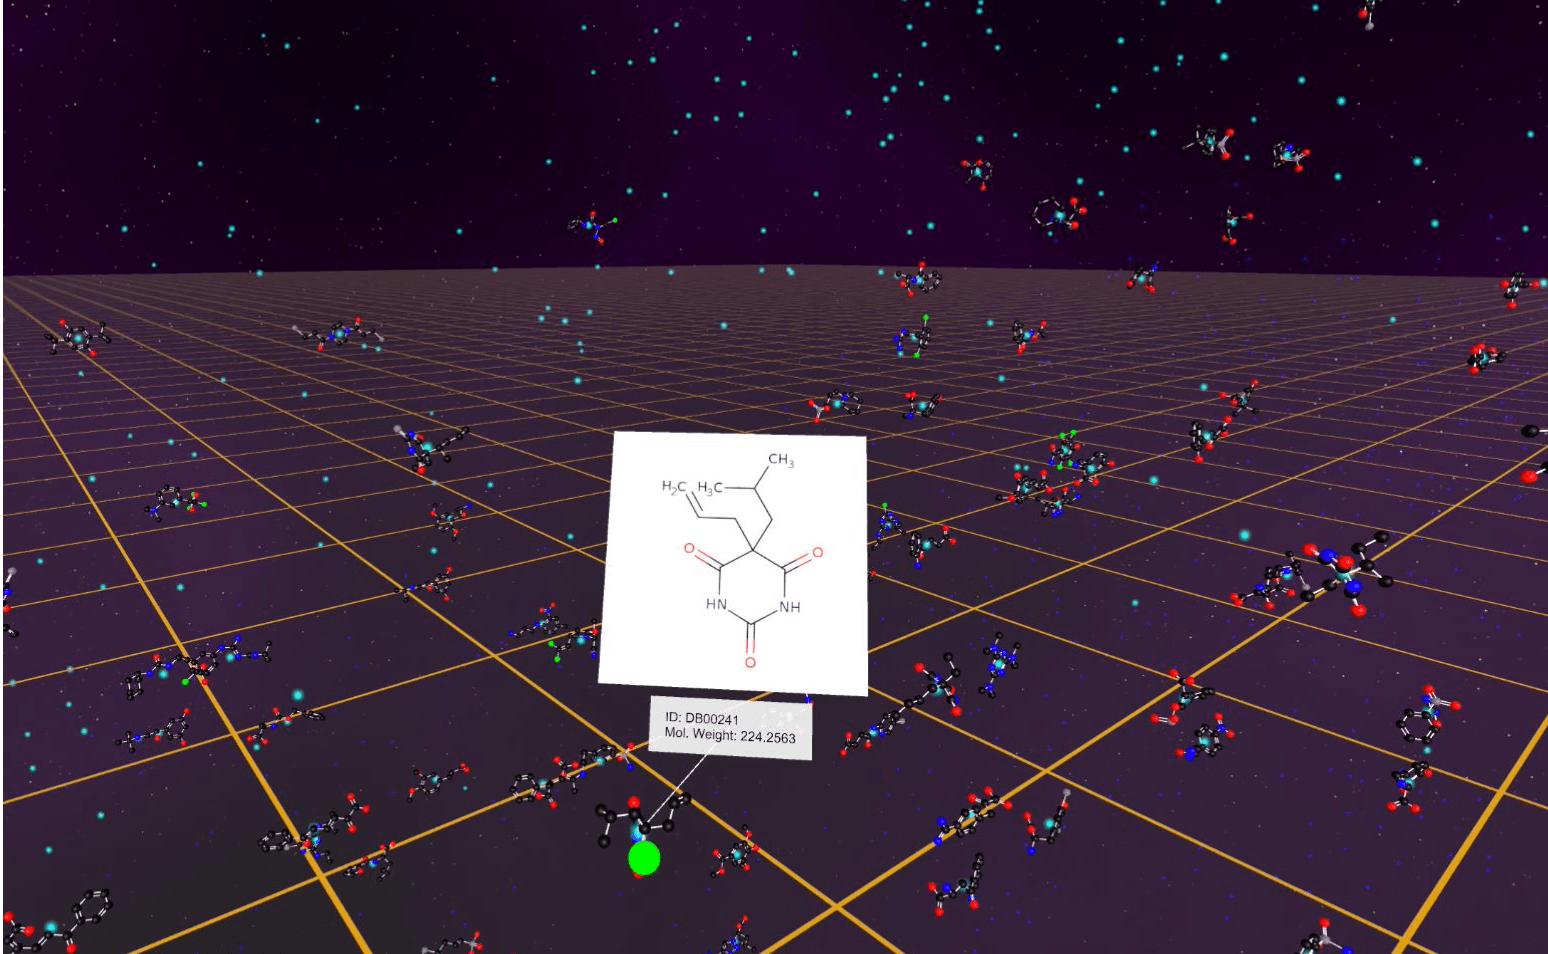
\includegraphics[width=\textwidth]{drugbank}
    \caption{Optimized virtual reality chemical space. Figure taken from \cite{drugbank}.}
    \label{fig:drugbank}
\end{figure}%

\section{BioVR}
BioVR is an interactive VR platform for integrated visual analysis of DNA/RNA protein structures\cite{biovr}. It is built in Unity and using C\#. The headset that they targeted the application to is Oculus Rift. One big difference between BioVR and our application is that in BioVR they use the hands for the interactions rather than the controllers. This can be very attractive and it could have worked very well for BigNet VR, since most of the interactions can be done with hand gestures. Also since early 2020, hand tracking has been integrated in Oculus Quest, making it easier for dveleopment\footnote{https://developer.oculus.com/documentation/unity/unity-handtracking}.
An screenshot of BioVR can be seen in Figure \ref{fig:biovr}. The user in BioVR can visualize the virtual hands in the virtual world and they are used for the interaction with the nucleotide sequence and UI menus. In BigNet VR instead of the hands we show the controllers, which help the user orientate in the space. The research concludes that using VR helps in create new workflows for researchers to view DNA/RNA sequence and protein structures. They also  of VR is that it is easy to integrate 2D user interfaces in the virtual world, as we can see in Figure \ref{fig:biovr} B.

\begin{figure}[h!]
    \centering%
    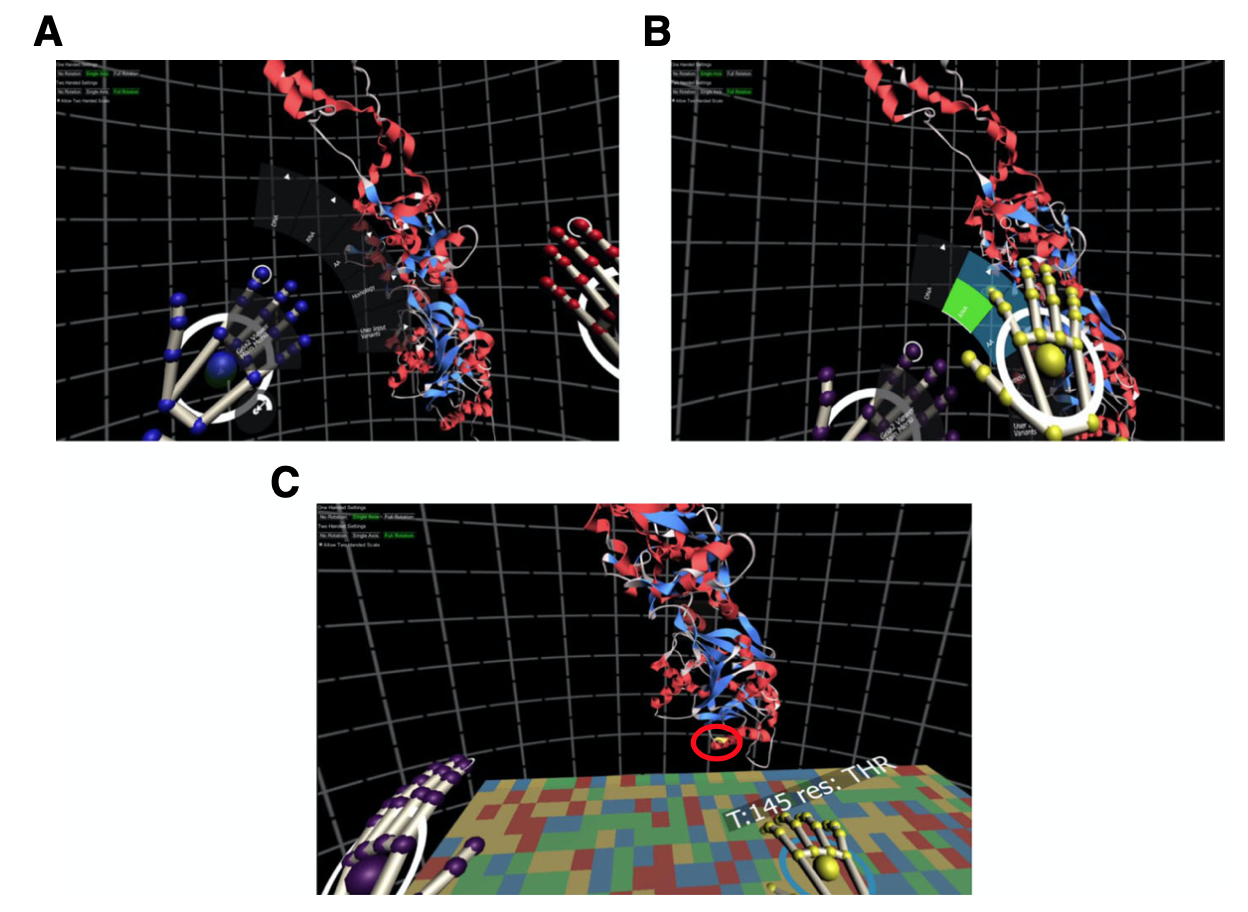
\includegraphics[width=\textwidth]{biovr}
    \caption{Screenshot from BioVR. Figure taken from \cite{biovr}.}
    \label{fig:biovr}
\end{figure}%

\section{CellexalVR}
CellexalVR is a virtual reality envirnoment for the visualization and analysis of single-cell RNAseq experiments that help researchers undertand their data\cite{cellexalvr}. The system is divided in two parts: the first one consists on the VR interface and the second is an R package called cellexalvrR that does back-end calculations and also provides functions that allows the user export the scRNAseq data from an R session for CellexalVR to read. CellexalVR was developed in Unity for HTC Vive (Pro). They used Unity and C\# and R for the implementation. They used libraries like VRTK, OpenVR and SteamVR as well in the implemenation.

Something that is interesting in CellexalVR is that it allows a multi-user mode via the Photon Unity Networking. This works sending information about the events to each user using Remote Procedure Calls. In Figure \ref{cellexavr} we can see an screenshot from CellexalVR where two users participate in the same session. Other users can also be in the same session but just be watchers and be in like a "ghost mode". This is something interesting that could be used in BigNet VR as well. Espcially the "ghost mode" could be useful so that other people can visualize the network at the same time from other perspectives.

\begin{figure}[h!]
    \centering%
    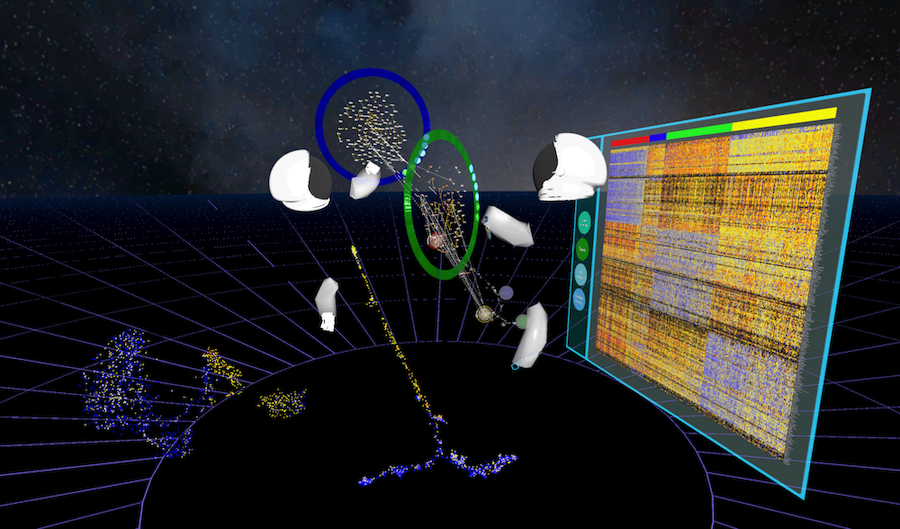
\includegraphics[width=\textwidth]{cellexavr}
    \caption{Screenshot from CellexalVR. Two users using CellexalVR at the same time. The head models were taken from NASA. Figure taken from \cite{cellexalvr}.}
    \label{fig:cellexavr}
\end{figure}%

\section{BigTop}
BigTop is a visualization framework in VR for the rendering of Manhattan plots in three dimensions\cite{bigtop}. Manhattan plots are usually 2-dimensionals, where genomic coordinates are displayed in the x-axis and the negative log-10 of the association P-value for each single nucleotide polymorphism (SNP) displayed on the Y-axis. Each dot on the Manhattan plot signifies a SNP then. In BigTop, the z-axis is used to display minor allele frequency of each SNP. This allows the identification of allelic variants of genes. As for the interaction, BigTop allows the user to select a node in order to obtain more information like the SNP name. BigTop is built in JavaScript with the React and A-Frame frameworks. It can also be rendered in any commercially available VR headsets and also in 2D web browsers.

To move around the scene in BigTop the user can take steps (in the VR version) or using the arrow keys from the keyboard. The user can select the nodes by pointing with a laser at the nodes in the scene in the VR version. In the browser version it is possible to select them using the pointer from the mouse. Also in order to look around, the user needs to move the head around using the VR headset, or by isong click and drag with the mouse (in the browser). In BigNet VR we have focused only into building a visualization system for a VR headset. We have used better locomotion techniques that improves the comfortability. However the locomotion technique that they use to move around could be a good idea for BigNet VR as well.

\begin{figure}[h!]
    \centering%
    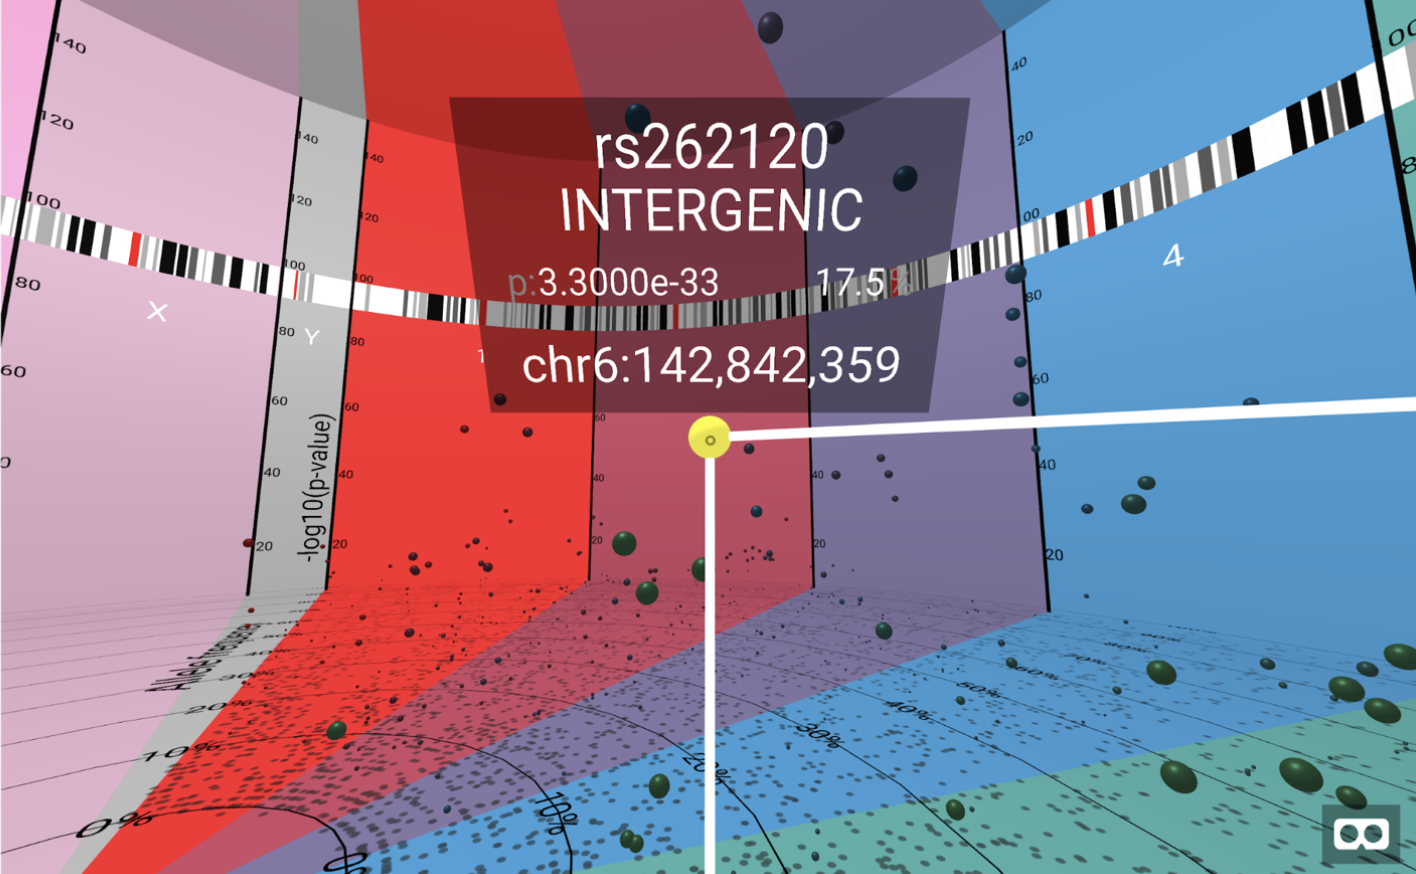
\includegraphics[width=\textwidth]{bigtop}
    \caption{Screenshot from BigTop. Figure taken from \cite{bigtop}.}
    \label{fig:bigtop}
\end{figure}%


\chapter{Conclusion}
We have developed GeneNet VR, a Virtual Reality application for the visualization of large biological networks. We used two datasets from MIxT, a real application with visualization problems, as a use case and solved scalability and information overload problems. GeneNet VR gives bioinformaticians the possibility to explore large biological networks for pattern identification using the Oculus Quest, a standalone economical VR headset.

Previous work for the visualization of large biological networks has shown common problems like the hairball problem, cumbersome interactions and scalability issues. We solve these in GeneNet VR by taking advantage of the rich interactivity that VR offers in order to balance out the amount of information. We have implemented several interaction and visualization techniques that help the users explore the large datasets. A locomotion system is used, providing the user a way to move around in the scene, solving also object occlusion problems common in 3D spaces. The user can also move the network around, zoom in it and filter the nodes using a 2-dimensional UI. The edges of the network are shown for each node when the user selects them using a laser pointer. Also, a novel feature allows the users compare two datasets in simultaneously.

We ran several performance experiments for our case study and demonstrated that GeneNet VR has a good performance when exploring the networks from MIxT. We also evaluated several interactions that are commonly used during the visualization process and achieved the required 72 FPS required by Oculus. We also evaluated the performance on the Oculus Quest hardware and the results indicated that the Oculus Quest is around 30\% slower than on the PC, but it is performs on 72 FPS.

We evaluated the quality of of our project with a qualitative research approach where we conducted purposive sampling with in-depth semi-structured interviews with research scientists from UiT. We obtained very good outstanding results, where the respondants highlighted that GeneNet VR is an interesting and useful tool to explore biological networks. The system is also easy to learn for the respondants event for those new to VR and the interactivity is smooth, making it easy to explore the networks. We also made a list with further requirements that we extracted from the interviews that will help us improve GeneNet VR in the future.

We believe that GeneNet VR is an important and useful tool for bioinformaticians. We have traced out the guidelines that enable VR as an affordable and advantageous option for the visualization of large biological networks. The rich interactivity that VR offers and the advancement in hardware has allowed us to solve visualization and scalability problems that are common in similar visualization tools. Now we ask ourselves, what are the next steps of GeneNet VR? And also, can we use a similar solution to visualize similar networks from other fields? Thanks to the interviews that we carried out, we think that GeneNet VR has potential in our research problem and can definitely be useful in other fields, for example for the visualization of drug and social networks.


\chapter{Future work}
GeneNet VR has room for improvements and new ideas. During the development, I used a git repository hosted on GitHub. I used the issues list that GitHub offers in order to have an overview of the problems that the application had. There are still a few issues opened and that I didn't have time to work with; some are bugs and others are ideas for future development. The project is now open source and anyone can contribute to it. The repository can be found in this URL on my GitHub account \footnote{https://github.com/kolibrid/GeneNet-VR}. The issue list can be found in this URL  \footnote{https://github.com/kolibrid/GeneNet-VR/issues}.

As we can see in the list, there are some issues that are tagged as "bug"; These bugs are not very big and don't prevent GeneNet VR from being functional. However, they have some impact on the usability of the application.

A problem that we found out is that when the application is run on the Oculus Quest hardware, the pointer for the 2D menu doesn't work. With this problem, the user cannot use the filters or the morph slider. Also when we morph the datasets, the new position of the networks is not taken into account if they have been translated previously. Other small bugs are that there seems to be an offset in the teleportation arrow, so the user doesn't teleport exactly to the direction of the arrow; also sometimes the pointer selects nodes that are behind the users, and it should be only the ones that are in front of the user.

We believe that GeneNet VR has also the potential for new development. We have written som ideas and tagged them with the word "enhancement" on GitHub. Something that could be interesting is to make the application multiuser. We got this idea from CellexalVR\cite{cellexalvr}, where two people can be in the same session and only one of them can interact with the data, the other is only a watcher. We could implement something similar in GeneNet VR, where one of the users is just a watcher but can for instance teleport to other parts of the network to visualize it.

Another improvement that we think that would enhance the performance of the application, is to create the lines that correspond to the edges during the initialization of the application and show them when they are needed. Right now, these lines are created in the scene every time a new node is selected. We use a function from Unity called Instantiate for this, which can downgrade the performance of the application, according to some forums from Unity.

Other improvements for BigNet VR would be focused on the aesthetics of the application. It's something that we haven't focused much in our prototype. An issue that we can see is that the nodes that we filter and that are morphed are turned into a black colour. It would be better to make the nodes transparent or to remove them from the network (when we filter them). If the nodes are still there but in black colour, they could hide other nodes that are behind them and the user might not see those nodes.

Other ideas that we had to improve GeneNet VR are for example highlight the nodes that are selected and their related nodes, the possibility to adjust the space between the nodes in the clusters and improve the 2D elements like the menu.

Finally, we would also like to run other experiments to further evaluate the performance of the application and study better the scalability. We would like to use larger datasets in order to determine where is the size limit for which we can visualize these datasets in GeneNet VR for both PC and the Oculus Quest headset.

\section{New requirements based on the interviews}
\begin{figure}[h!]
    \setlength{\tempheight}{15ex}
    \centering
    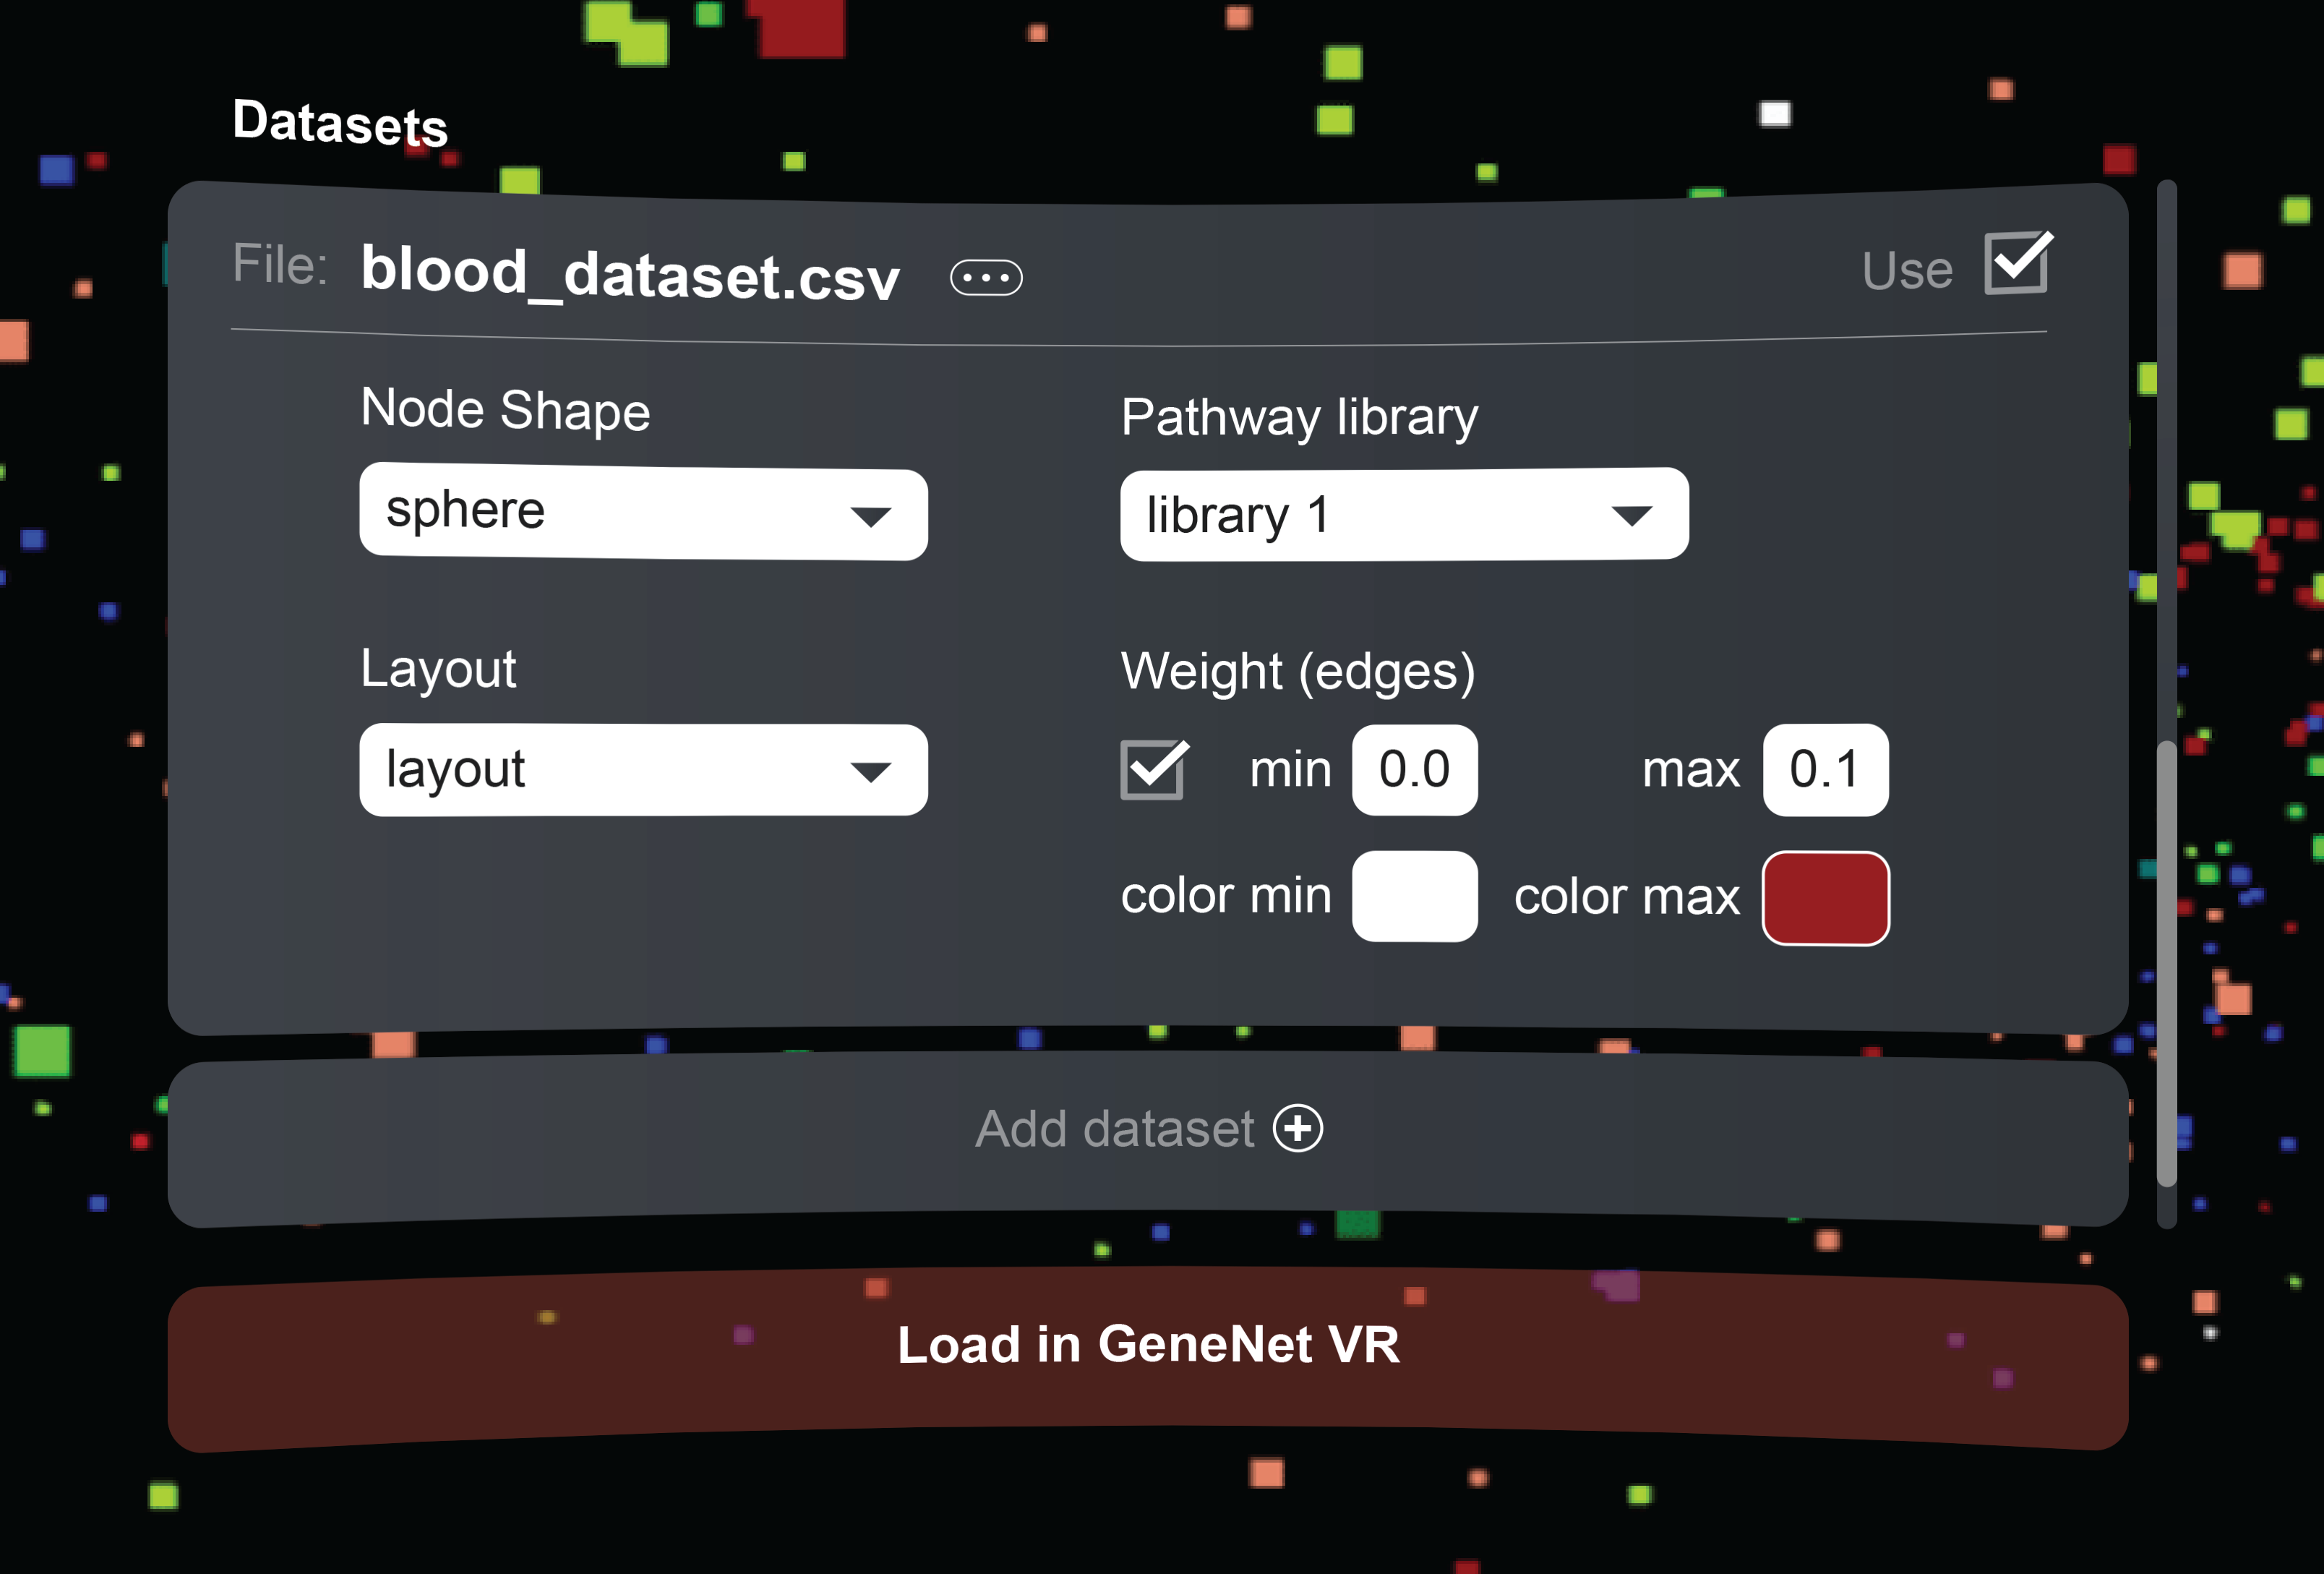
\includegraphics[width=\textwidth]{ui_future}
    \caption{Design of a user interface for GeneNet VR with help of a graphic designer.}
    \label{fig:issues}
\end{figure}

We obtained very interesting feedback from the interviews. We have created a list of issues based on this feedback and tagged them with the word "interviews" on GitHub.

Some respondents from the interviews who work on biology research projects claimed that it would be helpful to also see the names of the nodes that are interconnected to the selected node. When we select a node, we only get information for the node name that we have selected, but not for the interconnected nodes. A solution to this is to show a text label on the interconnected nodes or a small window with the interconnected node names. This task is tricky because we can end up having a lot of information. We can also try to highlight the nodes that we are visualizing and show the name labels when we get close to the nodes.

There is also information in the edges that we are not showing, as the weights. This information is common in networks like co-expression gene, social and drug networks. We can show the weight values by using a colour range in the lines or by changing the thickness of these. The distance between one and another node can also give important information about this.

Other improvements that we would like to do based on the interviews is: to be able to rotate the network with the controllers, filter the nodes by clusters, use a node search functionality, make the snap rotation smoother, be able to pin a node to compare it with other nodes and make it easier to select nodes by showing a collision circle around the nodes.

We also discussed the idea of building a notebook interface where the bioinformaticians can edit the datasets before uploading them to GeneNet VR. A notebook interface is a virtual notebook environment used for literate programming. It's a word processing tool where we also have a shell and kernel of a programming language. Notebooks are very useful to analyze data. The idea would be that the users can edit the dataset by changing the layout, using a different pathway library, changing the co-expression limit, adding other nodes, etc. then GeneNet CR is used to visualize the dataset by using the interaction functionalities.

Finally, we have created an improved user interface with some UI elements for GeneNet VR with help of a graphic designer, as we can see in Figure \ref{fig:issues}. These UI elements could be used in other parts of GeneNet VR like the filtering menu, a node search menu or to edit properties of the current network, to cite some examples.


\printbibliography

\begin{appendices}
\chapter{GitHub repository}
GeneNet VR is hosted on GitHub and can be accessed clicking on this URL: \url{https://github.com/kolibrid/GeneNet-VR}. The README file contains information about how to install the project and how to use it. The document uses the last version of the project with the following commit reference: \url{https://github.com/kolibrid/GeneNet-VR/commit/bd3908d689dae0ce2b5f31900e273bb996f1348d}.

We also made a video where we show the several interactions implemented for GeneNet VR. The video can be viewed on YouTube clicking on this link: \url{https://www.youtube.com/watch?v=\_Iqa3yizYZ4}.

\end{appendices}

\backmatter

\end{document}
